\documentclass[a4paper,12pt]{article}
\usepackage[a4paper,left=3cm,right=2cm,top=2cm,bottom=2cm]{geometry}
\usepackage{iftex}
\ifPDFTeX
\PackageError{IEEE_FULL_PAPER}{This report must be compiled with XeLaTeX}{Run xelatex IEEE_FULL_PAPER.tex from the docs/ directory.}
\fi
\usepackage{fontspec}
\setmainfont{Times New Roman}
\usepackage{unicode-math}
\setmathfont{Cambria Math}
\usepackage{setspace}
\setstretch{1.35}
\AtBeginDocument{\fontsize{13pt}{18.2pt}\selectfont}
\usepackage{fancyhdr}
\pagestyle{fancy}
\fancyhf{}
\fancyhead[C]{\thepage}
\renewcommand{\headrulewidth}{0pt}
\fancypagestyle{plain}{
  \fancyhf{}
  \fancyhead[C]{\thepage}
  \renewcommand{\headrulewidth}{0pt}
}
\setlength{\headheight}{16pt}
\usepackage{amsmath}
\usepackage{graphicx}
\usepackage{booktabs}
\usepackage{multirow}
\usepackage{array}
\usepackage{longtable}
\usepackage{algorithm}
\usepackage{algpseudocode}
\usepackage{siunitx}
\usepackage{enumitem}
\usepackage{float}
\usepackage{placeins}
\usepackage{etoolbox}
\usepackage{tocloft}
\usepackage{titlesec}
\usepackage{tikz}
\usetikzlibrary{arrows.meta,positioning,shapes.geometric,calc,fit,backgrounds}
\usepackage[unicode,hidelinks]{hyperref}
\setcounter{secnumdepth}{2}
\setcounter{tocdepth}{2}
\renewcommand{\thesection}{\arabic{section}}
\renewcommand{\thesubsection}{\thesection.\arabic{subsection}}
\renewcommand{\thesubsubsection}{\thesubsection.\arabic{subsubsection}}
\titleformat{\section}{\bfseries\fontsize{15}{20}\selectfont}{Chapter \thesection:}{0.6em}{}
\renewcommand{\contentsname}{Table of contents}
\renewcommand{\listtablename}{List of tables}
\renewcommand{\listfigurename}{List of figures}
\setlength{\cftsecnumwidth}{3.2em}
\setlength{\emergencystretch}{2em}
\makeatletter
\let\origsection\section
\renewcommand{\section}{%
  \@ifstar{\origsection*}{%
    \ifnum\value{section}>0
      \clearpage
      \thispagestyle{empty}\null\clearpage
    \else
      \clearpage
    \fi
    \origsection}%
}
\makeatother

\newcommand{\ReportTitle}{Dynamic Game State-Informed Fine-Tuned Language Models for Natural and Context-Aware NPC Dialogue in Narrative Games}
\newcommand{\ReportTitleVN}{Nâng cao tính tự nhiên và tính ngữ cảnh trong tương tác hội thoại với NPC bằng mô hình ngôn ngữ tinh chỉnh được thông tin bởi trạng thái thế giới game động trong game tường thuật}
\newcommand{\AuthorName}{Lê Trần Minh Phúc}
\newcommand{\AdvisorName}{TS. Lê Đăng Giáp}
\newcommand{\FacultyName}{Đào Tạo Đặc Biệt}
\newcommand{\StudentID}{2251010074}

\newcommand{\CoverPageBorder}{
\begin{tikzpicture}[remember picture,overlay]
\draw[line width=1.2pt]
  ([xshift=1cm,yshift=-1cm]current page.north west)
  rectangle
  ([xshift=-1cm,yshift=1cm]current page.south east);
\end{tikzpicture}
}
\newcommand{\ReportDate}{TP. Hồ Chí Minh, 2026}
\newcommand{\ProjectCode}{866}
\newcommand{\ind}{\mathbf{1}}
\newcommand{\BootstrapSamples}{5000}

\newcommand{\MainCoverPage}{
\begin{titlepage}
\thispagestyle{empty}
\CoverPageBorder
\begin{center}
{\large \textbf{BỘ GIÁO DỤC VÀ ĐÀO TẠO}}\\[0.3cm]
{\large \textbf{TRƯỜNG ĐẠI HỌC MỞ THÀNH PHỐ HỒ CHÍ MINH}}\\[2.5cm]
{\Large \textbf{BÁO CÁO TỔNG KẾT}}\\[0.4cm]
{\Large \textbf{ĐỀ TÀI NGHIÊN CỨU KHOA HỌC SINH VIÊN}}\\[1.2cm]
{\Large \textbf{\ReportTitleVN}}\\[2.4cm]
\vfill
{\LARGE \textbf{Mã số đề tài: \ProjectCode}}\\[2.0cm]
\vfill
\large \textbf{\ReportDate}
\end{center}
\end{titlepage}
}

\newcommand{\SecondaryCoverPage}{
\begin{titlepage}
\thispagestyle{empty}
\CoverPageBorder
\begin{center}
{\large \textbf{BỘ GIÁO DỤC VÀ ĐÀO TẠO}}\\[0.3cm]
{\large \textbf{TRƯỜNG ĐẠI HỌC MỞ THÀNH PHỐ HỒ CHÍ MINH}}\\[2.0cm]
{\Large \textbf{BÁO CÁO TỔNG KẾT}}\\[0.4cm]
{\Large \textbf{ĐỀ TÀI NGHIÊN CỨU KHOA HỌC SINH VIÊN}}\\[1.2cm]
{\Large \textbf{\ReportTitle}}\\[2.0cm]
\vfill
{\LARGE \textbf{Mã số đề tài: \ProjectCode}}\\[2.0cm]
\begin{minipage}{0.78\textwidth}
\centering
\large Chủ nhiệm đề tài: \AuthorName\\[0.4cm]
\large Khoa: \FacultyName\\[0.4cm]
\large Người hướng dẫn: \AdvisorName
\end{minipage}
\vfill
\large \textbf{\ReportDate}
\end{center}
\end{titlepage}
}

\newcommand{\ResultsInfoCoverPage}{
\begin{titlepage}
\thispagestyle{empty}
\begin{minipage}[t]{0.475\textwidth}
\centering
{\large \textbf{BỘ GIÁO DỤC VÀ ĐÀO TẠO}}\\[0.2cm]
{\large \textbf{TRƯỜNG ĐẠI HỌC MỞ}}\\[0.1cm]
{\large \textbf{THÀNH PHỐ HỒ CHÍ MINH}}
\end{minipage}
\hfill
\begin{minipage}[t]{0.475\textwidth}
\centering
{\large \textbf{CỘNG HOÀ XÃ HỘI CHỦ NGHĨA VIỆT NAM}}\\[0.2cm]
{\large \textbf{Độc lập - Tự do - Hạnh phúc}}
\end{minipage}

\vspace{1.2cm}
\begin{center}
{\Large \textbf{THÔNG TIN KẾT QUẢ NGHIÊN CỨU CỦA ĐỀ TÀI}}
\end{center}

\vspace{0.8cm}
\noindent\textbf{1. Thông tin chung:}\\
- Tên đề tài: \ReportTitleVN\\
- Tên đề tài (tiếng Anh): \ReportTitle\\
- Mã số đề tài: \ProjectCode\\
- Sinh viên chủ nhiệm đề tài: \AuthorName\\
- Khoa: \FacultyName \hfill Mã số sinh viên: \StudentID\\
- Giảng viên hướng dẫn: \AdvisorName

\vspace{0.45cm}
\noindent\textbf{2. Mục tiêu đề tài:}\\
Xây dựng và đánh giá một hệ thống hội thoại NPC tích hợp đầu-cuối cho trò chơi tường thuật, trong đó mô hình ngôn ngữ cục bộ được điều kiện hóa theo trạng thái trò chơi động nhằm nâng cao độ bám ngữ cảnh, tính nhất quán vai trò nhân vật và chất lượng phản hồi trong điều kiện triển khai thời gian thực.

\vspace{0.45cm}
\noindent\textbf{3. Tính mới và sáng tạo:}\\
Đề tài kết hợp đồng thời trích xuất ngữ cảnh từ UE5, truy hồi lai có cơ chế guard chống poisoning/trust-spoof, sinh phản hồi bằng mô hình tinh chỉnh cục bộ và lớp kiểm soát hậu sinh có cơ chế fallback trong cả hai nhánh triển khai Python và C++. Thiết kế này cho phép đồng nhất hành vi giữa môi trường đánh giá và runtime trong game, đồng thời hỗ trợ phân tích ablation theo từng thành phần.

\vspace{0.45cm}
\noindent\textbf{4. Kết quả nghiên cứu:}\\
Trên bộ 112 kịch bản cố định, cấu hình kiểm soát theo ngữ cảnh cải thiện có ý nghĩa thống kê so với cấu hình ngữ cảnh thô ở các chỉ số chính: context relevance (+0.1843), persona consistency (+0.1509), naturalness (+0.0967) và overall quality (+0.1440). Trong kiểm thử đối kháng, tỷ lệ tấn công thành công giảm từ 1.0 xuống 0.0 dưới cấu hình guard.

\vspace{0.45cm}
\noindent\textbf{5. Đóng góp về mặt kinh tế - xã hội, giáo dục và đào tạo, an ninh, quốc phòng và khả năng áp dụng của đề tài:}\\
Kết quả đề tài đóng góp quy trình kỹ thuật có thể kiểm chứng cho phát triển NPC hội thoại trong sản phẩm trò chơi số, hỗ trợ đào tạo liên ngành giữa AI và phát triển game, đồng thời nhấn mạnh cơ chế kiểm soát rủi ro nội dung khi ứng dụng mô hình ngôn ngữ trong hệ thống tương tác.

\vspace{0.45cm}
\noindent\textbf{6. Công bố khoa học của sinh viên từ kết quả nghiên cứu của đề tài:}\\
Hiện chưa có công bố khoa học chính thức; kết quả đang được hoàn thiện dưới dạng bản thảo học thuật và báo cáo kỹ thuật nội bộ.

\vfill
\begin{center}
{\large \textbf{\ReportDate}}
\end{center}
\end{titlepage}
}

\newcommand{\PrintAbbreviationList}{
\section*{List of abbreviations}
\phantomsection
\addcontentsline{toc}{section}{List of abbreviations}
\begin{center}
\begin{tabular}{p{0.18\textwidth}p{0.76\textwidth}}
\toprule
Abbreviation & Description \\
\midrule
ASR & Attack Success Rate \\
BM25 & Best Matching 25 retrieval model \\
CI & Confidence Interval \\
DPO & Direct Preference Optimization \\
LLM & Large Language Model \\
MRR & Mean Reciprocal Rank \\
nDCG & Normalized Discounted Cumulative Gain \\
NPC & Non-Player Character \\
OQ & Overall Quality \\
QLoRA & Quantized Low-Rank Adaptation \\
RAG & Retrieval-Augmented Generation \\
RQ & Research Question \\
TTFT & Time to First Token \\
UE5 & Unreal Engine 5 \\
\bottomrule
\end{tabular}
\end{center}
}

\begin{document}

\pagenumbering{gobble}
\MainCoverPage
\SecondaryCoverPage
\ResultsInfoCoverPage

\pagenumbering{roman}
\tableofcontents
\clearpage
\phantomsection
\addcontentsline{toc}{section}{List of tables}
\listoftables
\clearpage
\phantomsection
\addcontentsline{toc}{section}{List of figures}
\listoffigures
\clearpage
\PrintAbbreviationList
\clearpage
\pagenumbering{arabic}

\section*{Abstract}
\phantomsection
\addcontentsline{toc}{section}{Abstract}
This report presents an end-to-end NPC dialogue pipeline for narrative games that combines dynamic game-state grounding, guarded hybrid retrieval, local generation, and response control in Unreal Engine 5 across matched Python/C++ runtime paths. In a fixed 112-scenario benchmark, the controlled contextual system improves context relevance (+0.1843), persona consistency (+0.1509), naturalness (+0.0967), and overall quality (+0.1440) over raw contextual generation with paired-bootstrap support (\(p(\Delta \le 0)<1/\BootstrapSamples\), \(B=\BootstrapSamples\)). Human evaluation (324 ratings) provides pilot-scale preference evidence with moderate agreement (\(\kappa=0.5329\)). Guarded retrieval yields zero observed attack-follow cases (ASR 1.0\(\rightarrow\)0.0; exact 95\% upper bounds 0.0295 per set, 0.0149 pooled). The main limitation is serving efficiency and intervention burden (fallback 0.0089, retry 0.1071, first-pass acceptance 0.3750).

\section*{Keywords}
\phantomsection
\addcontentsline{toc}{section}{Keywords}
NPC dialogue, game AI, local LLM, UE5, QLoRA, response control, retrieval robustness, benchmark reproducibility, neuro-symbolic systems.

\section{Research problem, scope, and contributions}
This chapter defines the research problem and claim boundaries. It first clarifies why scripted pipelines and unconstrained LLM dialogue remain insufficient for deployment-critical narrative games, then specifies the study scope, research questions, and formal objective used in the rest of the report.
\subsection{Limitations of scripted and unconstrained NPC dialogue paradigms}
Narrative games require NPC dialogue that is simultaneously fluent, role-consistent, and grounded in dynamic world state. Survey evidence shows that classical authored dialogue pipelines remain dependable in production but incur rapidly growing authoring cost as interaction breadth increases \cite{Gallotta2024Survey,Sweetser2024Scoping}. LLM-driven NPC systems improve linguistic flexibility, yet often fail under strict gameplay constraints such as quest-state consistency, inventory grounding, and stable persona control across multi-turn interaction \cite{Park2023GenerativeAgents,Gallotta2024Survey,Sweetser2024Scoping}.

The core challenge is therefore not text generation alone; it is runtime integration. A model can produce plausible standalone responses and still behave unreliably in an engine loop when context extraction, retrieval ranking, and post-generation control are weakly coupled. Prior work demonstrates promising qualitative behavior, but system-level evidence is often limited by narrow scenario coverage, weak adversarial testing, or insufficient statistical reporting \cite{Gallotta2024Survey,Rao2024Minecraft}.

\subsection{Research focus: dynamic state-grounded local NPC dialogue in UE5}
This paper addresses that gap by designing and evaluating an end-to-end local runtime for context-grounded NPC dialogue in Unreal Engine 5. The method combines six components: bounded game-state serialization, prompt compilation, hybrid retrieval, guard-aware evidence scoring, local generation, and response control with fallback logic. The evaluation protocol is designed to answer a scientific question rather than present isolated demos: under fixed scenarios and controlled comparisons, does this architecture improve context relevance, persona consistency, and robustness without hiding negative trade-offs?

\subsection{Scope, assumptions, and boundary conditions}
The study is scoped to narrative-game dialogue under UE5 runtime constraints, with local model serving and fixed-scenario evaluation under matched prompts. The experimental window includes both adversarial stress settings and a predefined human-rating campaign so that automatic and human evidence are interpreted within the same protocol.

\subsection{Evidence strategy and inferential criteria}
To maintain scientific clarity, conclusions are explicitly scoped to measured axes. The study includes fixed-arm benchmarking, paired bootstrap tests, confidence intervals, ablations, human-rater agreement analysis, and adversarial stress evaluation. This design supports reporting both improvements (quality and security robustness) and limitations (serving latency/throughput trade-offs).

\subsection{Contributions and claim boundaries}
Relative to prior LLM-in-games studies, the main contribution is not local fine-tuning alone but the explicit coupling of architectural choices with inferential evidence. The report therefore states why each component is included, how it is evaluated, and which effects persist under ablation. This structure separates empirically supported engineering claims from hypotheses that require further study.

\subsection{Research questions}
The evaluation is organized around four explicit research questions. RQ1 examines whether controlled context-grounded inference improves context relevance, persona consistency, naturalness, and overall quality over raw contextual generation under matched prompts and decoding settings. RQ2 tests whether the same controlled setting yields a cross-condition quality gap relative to no-context external baselines under identical scenario protocols, without treating that contrast as isolated component attribution. RQ3 asks whether guard-aware retrieval materially reduces adversarial follow-through under poisoned and trust-spoofed evidence conditions. RQ4 characterizes the quality-latency trade-offs that emerge when guard and response-control mechanisms are enabled in an in-engine runtime.

\subsection{Formal objective and optimization formulation}
Formally, given player input \(x_t\), dynamic world state \(s_t\), retrieval corpus \(\mathcal{D}\), and NPC persona profile \(p\), the objective is to generate response \(y_t\) such that:
\begin{align}
\max\; &Q(y_t; x_t, s_t, p) \\
\text{s.t. } &R(y_t, s_t) \le \epsilon_r,\; C(y_t,p) \ge \tau_c,\; L(y_t) \le \tau_l,
\end{align}
where \(Q\) aggregates quality metrics, \(R\) denotes safety/risk violations, \(C\) denotes persona/context constraints, and \(L\) denotes runtime constraints.

For repeated interactions, the policy objective is:
\begin{equation}
\pi^\star=\arg\max_{\pi}\;\mathbb{E}_{(x_t,s_t,p)\sim\mathcal{T}}\left[Q\!\left(\pi(x_t,s_t,p)\right)\right],
\end{equation}
with quality decomposed as:
\begin{equation}
\begin{aligned}
Q &= w_{cr}CR + w_{pc}PC + w_nN + w_bB - w_vV,\\
\sum_i w_i &= 1,\quad w_i\ge0,
\end{aligned}
\end{equation}
where \(CR\) is context relevance, \(PC\) is persona consistency, \(N\) is naturalness, \(B\) is semantic similarity score, and \(V\) is violation risk. The empirical program then addresses four linked questions: whether controlled context-grounded inference improves over raw contextual generation, whether it yields a cross-condition gap relative to no-context external baselines under identical protocols, whether guard-aware retrieval reduces adversarial follow-through, and what serving trade-offs emerge when stronger control mechanisms are enabled. The contributions are therefore architectural, methodological, and empirical: an integrated UE5 runtime that combines state extraction, guarded hybrid retrieval, local generation, and runtime response control; parity between Python and C++ control paths; a fixed-arm benchmark with inferential statistics and multi-rater evaluation; and a reproducibility package that preserves both positive and negative findings.

For chapter-level traceability, Chapter 2 develops the theoretical and comparative grounding for these objectives, Chapter 3 defines the system and evaluation procedures used to test them, Chapter 4 reports quantitative and qualitative findings under that protocol, and Chapter 5 provides bounded conclusions and deployment-oriented recommendations.

\section{Theoretical and empirical foundations}
This chapter positions the study in the relevant literature and establishes the theoretical basis for the tested architecture. The discussion integrates international and Vietnamese research landscapes, then maps these foundations to explicit hypotheses evaluated in later chapters.
\subsection{International research landscape for LLM-driven game interaction}
Rule-based game dialogue systems remain strong in predictability and safety under strict authored quest logic, but their principal limitation is scalability because open-ended interaction breadth requires high authoring and maintenance cost \cite{Gallotta2024Survey,Sweetser2024Scoping}. LLM-driven NPC systems invert that trade-off by improving fluency and coverage, but they introduce instability under dynamic state constraints and longer interaction horizons \cite{Park2023GenerativeAgents,Gallotta2024Survey,Sweetser2024Scoping}. Recent interaction studies report promising collaboration and immersion signals while still documenting unresolved challenges in response latency, deterministic grounding, and robust runtime control \cite{Rao2024Minecraft,Christiansen2024Presence}. As a result, the central open problem has shifted from linguistic plausibility to controllable integration under game-runtime constraints.

Parallel work on game-capable language agents broadens this picture. Voyager demonstrates strong open-world progression in Minecraft through curriculum generation, skill-library reuse, and iterative code refinement \cite{Wang2023Voyager}. However, its objective is general embodied task completion rather than role-faithful NPC dialogue; consequently, it does not directly address persona consistency, narrative constraints, or dialogue-specific human preference evaluation. Similarly, SIMA emphasizes language-conditioned action execution across multiple 3D environments and shows progress on cross-world instruction following \cite{DeepMind2024SIMA}, but it is not designed as a narrative dialogue controller and therefore leaves unresolved the question of turn-level conversational admissibility under dynamic story state. At the interaction-interface level, voice-driven NPC systems can improve perceived freedom and engagement \cite{Wevelsiep2025Voice}; however, hybrid designs that map paraphrased speech to predefined dialogue options are intentionally constrained by authored dialogue structure, which limits fully open-ended generation under adversarial or contradictory context.

\subsection{Domestic research landscape and deployment context in Vietnam}
In Vietnam, the VLSP community has provided a sustained research backbone through shared tasks, benchmark construction, and reproducible evaluation workflows across language and speech problems \cite{VLSP2025Proceedings,Ha2025VLSPSemanticParsing}. Recent work has expanded this foundation toward Vietnamese large-model development, including foundation-model adaptation and language-specific continual pretraining such as VinaLLaMA and Vi-Mistral-X \cite{VinaLLaMA2023,ViMistralX2024}. In parallel, early Vietnamese RAG and multimodal-LLM studies have improved resource availability through open datasets, evaluation suites, and model releases \cite{Duc2024VietnamRAG,LaVy2024}.

These advances, however, are still concentrated in general NLP capability, benchmark engineering, and modality expansion, rather than in audited in-engine NPC dialogue systems that combine dynamic game-state grounding, adversarial retrieval controls, and runtime-parity validation. The domestic gap addressed here is therefore system integration under deployment constraints, not base-model capability alone.

\subsection{Core constructs and operational definitions}
This work uses four central concepts: context relevance as fidelity to dynamic world state, persona consistency as adherence to NPC role profile, naturalness as linguistic plausibility under interaction constraints, and robustness as resistance to malicious or inconsistent evidence injection.

\subsection{Theoretical foundations for adaptation, retrieval, and runtime control}
At the model-adaptation level, prompt engineering and instruction tuning provide fast behavior shaping \cite{Liu2021PromptSurvey}, while RLHF-style methods and preference optimization improve adherence to desired responses \cite{Ouyang2022InstructGPT,Rafailov2023DPO}. Prompting strategies that explicitly structure intermediate reasoning and action feedback, such as Chain-of-Thought and ReAct, further strengthen controllability in complex task settings \cite{Wei2022CoT,Yao2023ReAct}. Parameter-efficient adaptation through LoRA and QLoRA enables local deployment under constrained memory budgets \cite{Hu2021LoRA,Dettmers2023QLoRA}. Retrieval-aware generation frameworks such as Self-RAG further show that adaptive retrieval and self-critique can improve factuality \cite{Asai2024SelfRAG}. Their main weakness for deployment-critical NPC systems is that they prioritize general factual quality and controllability, but do not explicitly target adversarial evidence handling in game-specific retrieval pipelines.

Benchmarking work on LLM agents and long-context reasoning clarifies why these gaps persist in runtime game deployments. AgentBench shows that even strong models degrade on multi-turn decision tasks requiring sustained planning and instruction fidelity \cite{Liu2023AgentBench}. LongBench further shows that performance drops substantially as context length and task heterogeneity increase, and that retrieval-based compression only partially closes the gap for weaker long-context models \cite{Bai2024LongBench}. For dynamic NPC dialogue, these findings imply that naive context accumulation is insufficient; bounded state serialization, retrieval prioritization, and explicit post-generation control are required to maintain stable behavior as interaction horizons expand.

Retrieval-augmented generation strengthens factual grounding, from the original RAG formulation to later survey syntheses and graph-based extensions \cite{Lewis2020RAG,Fan2024RAGSurvey,Edge2024GraphRAG}. However, retrieval also creates a new control surface where poisoning, trust spoofing, and ranking manipulation can alter downstream generation. Recent high-impact attack studies reinforce this concern: indirect prompt injection can compromise application behavior through retrieved context \cite{Greshake2023PromptInjection}, knowledge-corruption attacks can induce attacker-chosen outputs with a small number of injected passages \cite{Zou2025PoisonedRAG}, and adversarial instructional prompts can subvert retrieval behavior even when user queries are fixed \cite{Chaturvedi2025AIP}. A substantial share of reported evaluations remains centered on benign relevance quality, while adversarial coverage is less consistently reported in game-oriented dialogue settings. This is a key weakness for game NPC settings, where retrieval errors can directly induce in-character policy violations. Evaluation methodology presents a related issue: overlap-only scoring is insufficient for interactive dialogue quality, dialog-metric behavior can vary substantially across datasets and settings \cite{Yeh2021DialogMetrics}, and modern embedding- and judge-based protocols can still carry positional or verbosity biases \cite{Zhang2020BERTScore,Zheng2023MTBench,Wang2024Judge,Dubois2024AlpacaEval}. For this reason, interactive dialogue systems require convergent evidence across automatic metrics, inferential statistics, human preference, and agreement analysis \cite{Cohen1960Kappa}.

\subsection{Hypotheses and analytical model}
The integrated theoretical position tested in this report is that coupling guarded retrieval and response control with dynamic game-state conditioning produces measurable gains in relevance, persona fidelity, and robustness under fixed evaluation constraints.

Operationally, this position is tested through four linked hypotheses aligned with the research questions: controlled context-grounded inference improves core quality metrics over raw contextual inference; the same controlled setting yields a cross-condition quality gap over no-context external baselines under matched protocols; guarded retrieval reduces adversarial follow-through probability; and the quality and robustness gains are accompanied by measurable serving-time overhead. These hypotheses are evaluated with paired comparisons and uncertainty reporting rather than point estimates alone, with cross-condition comparisons treated as system-level diagnostics rather than isolated component-causality tests.

The gap addressed in this paper is therefore not a missing individual component but a missing systems integration with strong inferential discipline. This chapter provides scoped comparative positioning against representative prior systems \cite{Gallotta2024Survey,Sweetser2024Scoping,Rao2024Minecraft}, rather than an exhaustive novelty determination. The present study is positioned as a fixed-protocol integration test, and its conclusions are bounded to measured axes rather than broad model-general assertions.
To make this statement auditable, the review scope was restricted to January 2020--February 2026 and prioritized indexed records in IEEE Xplore, ACM Digital Library, ACL Anthology, and arXiv, with predefined keyword families spanning NPC dialogue, game-state grounding, retrieval control/guarding, and in-engine runtime evaluation. Query templates and inclusion/exclusion rules are reported in Appendix A; this was a targeted review, not a full systematic-review protocol.

\begin{table}[t]
\centering
\caption{Comparative positioning snapshot against representative prior systems.}
\label{tab:chapter2_positioning}
\begingroup
\footnotesize
\setlength{\tabcolsep}{3pt}
\resizebox{\textwidth}{!}{%
\begin{tabular}{lccccc}
\toprule
Representative system & Dynamic game-state grounding & Retrieval attack handling & Runtime parity checks & Inferential + human evidence & Limitation relative to this study \\
\midrule
Generative Agents \cite{Park2023GenerativeAgents} & Partial & No & No & Limited & Focuses on social simulation rather than in-engine constraint control \\
Minecraft NPC collaboration \cite{Rao2024Minecraft} & Partial & No & Limited & Limited & Emphasizes interaction quality, with narrower robustness analysis \\
Voyager \cite{Wang2023Voyager} & No (dialogue-centric) & No & Limited & No & Optimizes task progression, not persona-grounded NPC dialogue reliability \\
Self-RAG \cite{Asai2024SelfRAG} & No (game-runtime specific) & Limited & No & Partial & Strong retrieval generation quality, but not game-runtime adversarial integration \\
This study & Yes & Yes & Yes & Yes & Latency and throughput remain weaker than lightweight baselines \\
\bottomrule
\end{tabular}}
\endgroup
\end{table}

\subsection{Novelty decomposition and evidence-backed differentiation}
To make novelty claims auditable, Table~\ref{tab:novelty_decomposition} decomposes the proposed contribution into concrete technical elements and maps each element to direct empirical evidence in this report. This avoids a generic ``end-to-end system'' claim and clarifies which parts are demonstrated versus only proposed for future work.

\begin{table}[t]
\centering
\caption{Novelty decomposition mapped to direct evidence in this report.}
\label{tab:novelty_decomposition}
\begingroup
\footnotesize
\setlength{\tabcolsep}{3.5pt}
\begin{tabular}{p{0.24\textwidth}p{0.26\textwidth}p{0.19\textwidth}p{0.24\textwidth}}
\toprule
Technical element & Differentiation in this study & Evidence status & Direct evidence location \\
\midrule
UE5 state-grounded dialogue binding & Explicit behavior-tree trigger path, blackboard key serialization, async inference boundary, timeout/fallback control in one runtime description & Demonstrated & Sec. 3.2 and Sec. 3.3; Tables~\ref{tab:ue5_operational_metrics}--\ref{tab:ue5_state_operational} \\
Guard-aware hybrid retrieval for NPC dialogue & Retrieval relevance combined with poisoning/trust-spoof risk penalty in ranking objective & Demonstrated & Guarded score definition in Sec. 3.2 and adversarial results in Sec. 4.3 \\
Dual-path runtime parity & Matched Python and C++ response-control behavior to reduce benchmark/runtime divergence risk & Demonstrated & Sec. 3.2 and Appendix (Response-control specification) \\
Evidence-gated reporting protocol & Conjunctive gate requiring coverage, significance, human, retrieval, and security evidence before pass status & Demonstrated & Sec. 3.1, Algorithm 1 \\
Operationally adaptive control thresholds by UE5 state & State-conditioned threshold/retry-budget policy to reduce fallback/retry burden while preserving safety caps & Proposed next upgrade & Sec. 3.4 and Sec. 5.4 \\
\bottomrule
\end{tabular}
\endgroup
\end{table}

\section{System architecture and empirical methodology}
This chapter reports the end-to-end research procedure and the mixed-method design used in the study, combining quantitative fixed-arm evaluation with qualitative scenario-level interpretation and rater-based judgment.

\subsection{Evidence-gating protocol and study design}
The evaluation protocol is defined as an evidence-completeness criterion rather than a binary yes-or-no decision rule. Let:
\begin{equation}
\Gamma = \ind\!\left[C_{cov}\land C_{sig}\land C_{human}\land C_{retr}\land C_{sec}\right],
\end{equation}
where \(C_{cov}\) is scenario coverage, \(C_{sig}\) is controlled-vs-raw significance, \(C_{human}\) is human-evaluation completeness and agreement, \(C_{retr}\) is retrieval reporting completeness, and \(C_{sec}\) is adversarial-security performance.

Under this definition, \(\Gamma=1\) indicates that all required evidence components are present, while \(\Gamma=0\) indicates that at least one component is missing. Core requirements include minimum scenario coverage of 100 (achieved: 112), significant controlled-vs-raw improvements on key quality metrics, completed human-evaluation requirements (including row count, agreement, and preference checks), complete reproducibility artifacts (metadata, retrieval metrics, ablations, and confidence intervals), and security criteria based on ASR reduction and guarded-ASR caps. Cross-condition external-baseline comparisons are reported as non-gating diagnostics.

This protocol is necessary because game-AI reports often conflate demonstration quality with deployment reliability. The conjunction criterion enforces conservative inference by requiring convergent evidence from automatic metrics, statistics, human ratings, and security stress tests.

Formally, with \(C_j\in\{0,1\}\), \(\Gamma\) is equivalent to a product gate:
\begin{equation}
\Gamma=\prod_{j\in\{cov,sig,human,retr,sec\}} C_j.
\end{equation}
Hence \(\Gamma=1\) if and only if all gating components equal \(1\), and any missing gating component forces \(\Gamma=0\). This gives the gate a conservative monotonic property: strengthening a component from \(0\) to \(1\) cannot reduce \(\Gamma\), while any remaining \(0\) still blocks a pass. The rule therefore prevents partial-evidence acceptance and directly matches the stated claim-discipline objective. In Algorithm 1, \(\mathcal{B}_{ext}\) denotes the set of external no-context baselines included in the benchmark (here: phi3:mini and phi3:latest), used for non-gating cross-condition diagnostics.

\begin{algorithm}[H]
\caption{Evidence-completeness gate evaluation}
\begin{algorithmic}[1]
\Require benchmark summary \(\mathcal{B}\), retrieval report \(\mathcal{R}\), human report \(\mathcal{H}\), security report \(\mathcal{S}\)
\Require core metric set \(\mathcal{M}_{core}\), significance level \(\alpha\)
\Require thresholds \((n_{min},\kappa_{min},\rho_{min},a_{max})\)
\State \(C_{cov}\gets \ind(\mathcal{B}.\text{scenario\_count}\ge n_{min})\)
\State \(C_{sig}\gets \ind\!\Big(\forall m\in\mathcal{M}_{core}: p_m\le\alpha \land CI_{m,\Delta}^{L}>0\Big)\)
\State \(D_{base}\gets \ind\!\Big(\forall b\in\mathcal{B}_{ext}: \Delta OQ_b>0 \land CI^{L}_{\Delta OQ,b}>0\Big)\) \Comment{non-gating diagnostic}
\State \(C_{human}\gets \ind(\mathcal{H}.\text{ratings complete} \land \mathcal{H}.\kappa\ge\kappa_{min})\)
\State \(C_{retr}\gets \ind(\mathcal{R}.\text{metrics and ablations complete})\)
\State \(C_{sec}\gets \ind(\mathcal{S}.\Delta_{ASR}\ge\rho_{min} \land \mathcal{S}.ASR_{guard}\le a_{max})\)
\State \(\mathcal{J}\gets\{cov,sig,human,retr,sec\}\)
\State \(\Gamma \gets C_{cov}\cdot C_{sig}\cdot C_{human}\cdot C_{retr}\cdot C_{sec}\)
\State \Return \(\Gamma\), \(\{j\in\mathcal{J}: C_j=0\}\), and \(D_{base}\) as non-gating cross-condition diagnostic
\end{algorithmic}
\end{algorithm}

\subsection{Online runtime architecture and data flow}

The runtime pipeline is organized into six sequential stages: context extraction from UE5 simulation state, prompt and query construction with persona and dynamic-context slots, hybrid retrieval with guard-aware evidence scoring, local LLM generation, response-control rewrite or fallback selection, and memory-plus-citation updates. This decomposition was selected to isolate failure modes that are otherwise entangled in monolithic prompting pipelines. In particular, extraction errors, retrieval errors, and generation errors can be inspected independently, which improves both debugging and ablation interpretability.

The architecture is implemented across engine-runtime and Python orchestration layers with explicit parity checks for core response-control behavior. This implementation choice addresses a common validity risk in LLM systems for games: benchmark behavior diverges from runtime behavior when evaluation logic and deployment logic are maintained in separate code paths.

\begin{figure}[t]
\centering
\resizebox{0.96\textwidth}{!}{%
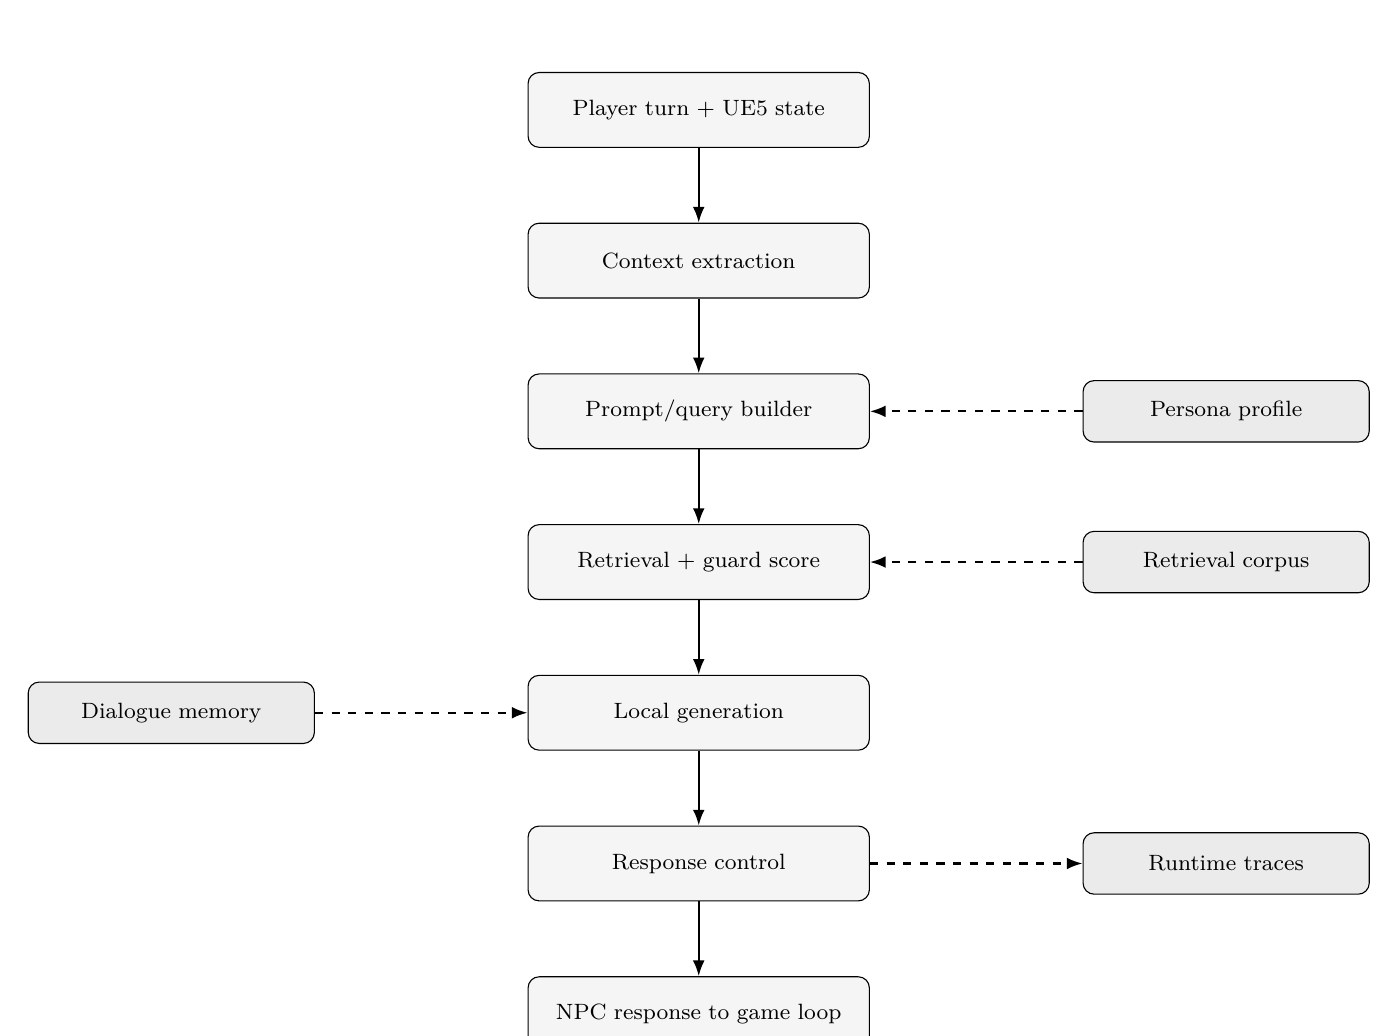
\begin{tikzpicture}[
  font=\footnotesize,
  node distance=0.95cm,
  module/.style={draw, rounded corners, minimum height=0.95cm, text width=4.1cm, align=center, fill=gray!8},
  store/.style={draw, rounded corners, minimum height=0.78cm, text width=3.4cm, align=center, fill=gray!16},
  flow/.style={-{Latex[length=2mm]}, thick},
  aux/.style={-{Latex[length=2mm]}, thick, dashed},
  note/.style={font=\scriptsize, align=left}
]
\node[module] (input) {Player turn + UE5 state};
\node[module, below=of input] (ctx) {Context extraction};
\node[module, below=of ctx] (prompt) {Prompt/query builder};
\node[module, below=of prompt] (retr) {Retrieval + guard score};
\node[module, below=of retr] (llm) {Local generation};
\node[module, below=of llm] (ctrl) {Response control};
\node[module, below=of ctrl] (out) {NPC response to game loop};

\node[store, right=2.7cm of prompt] (persona) {Persona profile};
\node[store, right=2.7cm of retr] (corpus) {Retrieval corpus};
\node[store, left=2.7cm of llm] (memory) {Dialogue memory};
\node[store, right=2.7cm of ctrl] (telemetry) {Runtime traces};

\draw[flow] (input) -- (ctx);
\draw[flow] (ctx) -- (prompt);
\draw[flow] (prompt) -- (retr);
\draw[flow] (retr) -- (llm);
\draw[flow] (llm) -- (ctrl);
\draw[flow] (ctrl) -- (out);

\draw[aux] (persona.west) -- (prompt.east);
\draw[aux] (corpus.west) -- (retr.east);
\draw[aux] (memory.east) -- (llm.west);
\draw[aux] (ctrl.east) -- (telemetry.west);
\end{tikzpicture}%
}
\caption{Online runtime architecture and data flow. Solid arrows denote inference flow; dashed arrows denote conditioning and control inputs.}
\label{fig:runtime_architecture}
\end{figure}

\begin{figure}[t]
\centering
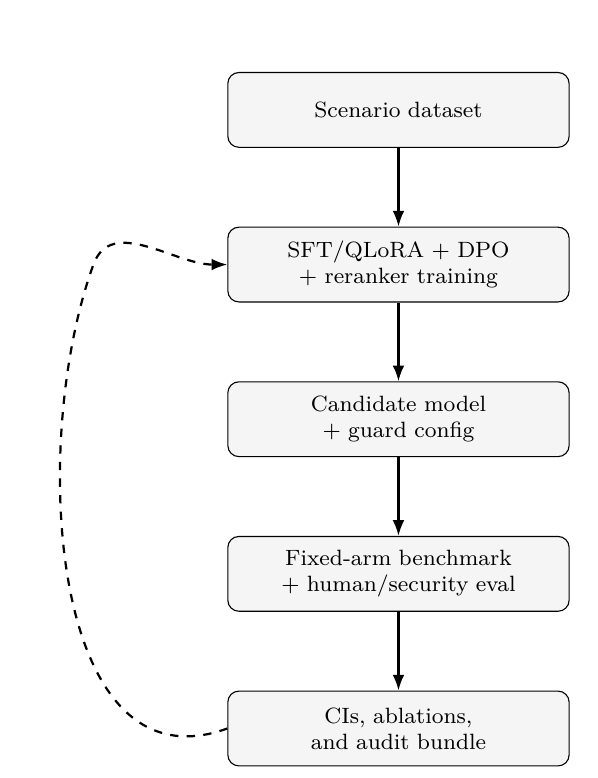
\begin{tikzpicture}[
  font=\footnotesize,
  node distance=1.0cm,
  module/.style={draw, rounded corners, minimum height=0.95cm, text width=4.1cm, align=center, fill=gray!8},
  flow/.style={-{Latex[length=2mm]}, thick},
  aux/.style={-{Latex[length=2mm]}, thick, dashed}
]
\node[module] (scenario) {Scenario dataset};
\node[module, below=of scenario] (train) {SFT/QLoRA + DPO + reranker training};
\node[module, below=of train] (candidate) {Candidate model + guard config};
\node[module, below=of candidate] (bench) {Fixed-arm benchmark + human/security eval};
\node[module, below=of bench] (artifact) {CIs, ablations, and audit bundle};

\draw[flow] (scenario) -- (train);
\draw[flow] (train) -- (candidate);
\draw[flow] (candidate) -- (bench);
\draw[flow] (bench) -- (artifact);

\draw[aux] (artifact.west) to[out=200,in=250] ([xshift=-1.7cm]train.west) to[out=70,in=180] (train.west);
\end{tikzpicture}
\caption{Offline training and evaluation flow with feedback loops. The candidate model and control configuration are exported to the online runtime pipeline in Figure~\ref{fig:runtime_architecture}.}
\label{fig:offline_pipeline}
\end{figure}

The online execution path in Figure~\ref{fig:runtime_architecture} is coupled with the offline build-and-validate path in Figure~\ref{fig:offline_pipeline}. This coupling is deliberate: the model, guard configuration, and evaluation artifacts are produced offline and then transferred into runtime under parity checks, reducing benchmark-versus-deployment drift.

The UE5 context extractor serializes behavior state, zone or location features, nearby entities, and recent event summaries. Instead of injecting unbounded world logs, it uses bounded payloads and normalized keys. This design is chosen over direct transcript-style context injection because game-state grounding depends on precise key-value consistency, while free-form logs often waste context budget on low-value narrative details. Bounded serialization therefore reduces prompt explosion, preserves critical quest and inventory fields, and enables stable prompt templates under fixed token budgets.

The retriever combines sparse matching (BM25-like lexical) and dense similarity. Candidate evidence is re-ranked with a guard-aware score:
\begin{equation}
s_i = \alpha s_i^{dense} + (1-\alpha)s_i^{sparse} - \lambda g_i,
\end{equation}
where \(g_i\) is a risk term that aggregates injection cues, trust-spoof likelihood, and metadata inconsistency. The hybrid form is selected because sparse matching is reliable for exact in-game entities, while dense retrieval improves recall for paraphrased player input; neither method alone is consistently robust across both cases. Guard-aware re-ranking is added because standard relevance scoring assumes benign documents and can over-rank adversarial text that imitates authority, a behavior consistent with recent poisoning and adversarial-instruction results in retrieval pipelines \cite{Zou2025PoisonedRAG,Chaturvedi2025AIP}. The resulting score discourages high-ranked poisoned evidence without disabling retrieval utility.

Response control performs post-generation checks and optional rewrite/select logic. It is implemented in both Python and C++ paths to guarantee runtime parity between evaluation and in-game behavior. For candidate output \(\hat{y}\), the controller computes:
\begin{equation}
F(\hat{y}) = w_c\phi_c + w_p\phi_p + w_n\phi_n - w_v\phi_v.
\end{equation}
If \(F(\hat{y}) < \tau\), the system triggers a grounded fallback policy rather than returning unstable free-form text. This stage is included as a runtime alignment layer complementary to training-time adaptation, because instruction tuning and preference optimization improve average behavior but cannot guarantee turn-level admissibility under noisy or adversarial context.

The guard weight \(\lambda\) and control threshold \(\tau\) are selected by constrained calibration on a development set. The calibration objective is to maximize dialogue quality while enforcing robustness and admissibility caps, rather than tuning to quality alone.

\begin{algorithm}[H]
\caption{Guard-threshold calibration under risk constraints}
\begin{algorithmic}[1]
\Require development scenario set \(\mathcal{S}_{dev}\), candidate grids \(\Lambda,\mathcal{T}_{\tau}\)
\Require risk cap \(a_{max}\), optional fallback-rate cap \(f_{max}\), latency weight \(\eta\)
\State initialize \(J^\star\gets-\infty\), \(T^\star\gets+\infty\), best pair \((\lambda^\star,\tau^\star)\gets(\text{None},\text{None})\)
\For{each \(\lambda\in\Lambda\)}
  \For{each \(\tau\in\mathcal{T}_{\tau}\)}
    \State run guarded pipeline on \(\mathcal{S}_{dev}\) with \((\lambda,\tau)\)
    \State compute mean quality \(\bar{Q}\), \(ASR_{guard}\), fallback rate \(F_{rate}\), and latency \(T\)
    \If{\(ASR_{guard}\le a_{max}\) and (\(F_{rate}\le f_{max}\) or no fallback cap)}
      \State compute calibration utility \(J\gets \bar{Q}-\eta T\)
      \If{\(J>J^\star\) or (\(J=J^\star\) and \(T<T^\star\))}
        \State update \((J^\star,T^\star,\lambda^\star,\tau^\star)\gets(J,T,\lambda,\tau)\)
      \EndIf
    \EndIf
  \EndFor
\EndFor
\If{\((\lambda^\star,\tau^\star)=(\text{None},\text{None})\)}
  \State \Return fail-closed (no feasible pair under current caps; relax grid or constraints)
\EndIf
\State \Return \((\lambda^\star,\tau^\star)\)
\end{algorithmic}
\end{algorithm}

\begin{algorithm}[H]
\caption{Runtime inference with guarded response control}
\begin{algorithmic}[1]
\Require player input $x_t$, world state $s_t$, persona $p$, retrieval corpus $\mathcal{D}$
\State $c_t \gets \textsc{ExtractContext}(s_t)$
\State $q_t \gets \textsc{BuildRetrievalQuery}(x_t,c_t,p)$
\State $E_t \gets \textsc{HybridRetrieve}(q_t,\mathcal{D})$
\State $\tilde{E}_t \gets \textsc{GuardFilter}(E_t)$
\State $\pi_t \gets \textsc{BuildPrompt}(x_t,c_t,p,\tilde{E}_t)$
\State $\hat{y}_t \gets \textsc{GenerateLocal}(\pi_t)$
\State $y_t \gets \textsc{ResponseControl}(\hat{y}_t, x_t, c_t, p)$
\State \textsc{UpdateMemoryAndCitations}$(y_t,\tilde{E}_t)$
\State \Return $y_t$
\end{algorithmic}
\end{algorithm}

The algorithm has a stagewise cost decomposition
\begin{equation}
T_{total}=T_{ctx}+T_{ret}+T_{guard}+T_{gen}+T_{ctrl}+T_{mem}.
\end{equation}
With top-\(M\) retrieved candidates, guard scoring is \(O(M)\), while generation dominates asymptotically through autoregressive decoding. This decomposition explains the observed latency trade-off: robustness and admissibility checks increase deterministic overhead even when generation settings are fixed.

\subsection{UE5 execution binding: behavior-tree triggers, state serialization, and latency control}
In the UE5 runtime, dialogue generation is invoked through \texttt{RequestResponse} in \texttt{UNPCDialogueComponent}, typically from interaction logic or behavior-tree task transitions when an NPC enters a speak-eligible state. At invocation time, the component snapshots live world context and forwards generation to \texttt{GenerateDialogueAsync} in \texttt{UNPCInferenceSubsystem}. Inference executes on a UE5 background worker thread in the \texttt{AnyBackgroundThread} family, while completion callbacks are marshaled back to the game thread (\texttt{GameThread}) \cite{EpicGames2025TaskGraph,EpicGames2025EAsyncExecution}. This split keeps simulation and rendering responsive while preserving deterministic game-thread updates for animation, UI, and dialogue state progression.

State serialization is anchored in AI-controller telemetry rather than free-form logs. The extractor records the active behavior-tree node (\path|CurrentBehavior|), a normalized behavior state (\path|BehaviorState|), and non-empty blackboard entries (\path|BlackboardValues|). Common keys include \path|IsAlerted|, \path|IsPatrolling|, and \path|IsInCombat|. It also serializes zone/location, nearby entities, perception signals (visible/heard actors, player visibility), time/weather, and recent events. The serialized payload is bounded and normalized before prompt compilation so that retrieval and generation are conditioned on explicit runtime state, consistent with Unreal Engine's documented Behavior Tree and Blackboard model \cite{EpicGames2025UEBehaviorTrees}.

Latency governance combines transport-level bounds with gameplay-level freshness control. The transport path enforces request timeouts (30 s in the inference client transport; 180 s in the benchmark harness), while gameplay logic suppresses stale completions by canceling in-flight generation if interaction context changes, for example when the player leaves the interaction envelope during generation. If first-pass output is empty or fails response-control admissibility checks, the runtime applies rewrite attempts and then a grounded fallback response.

Operational runtime metrics are defined as:
\begin{align}
\mathrm{TimeoutRate} &= \frac{N_{timeout}}{N_{turn}},\\
\mathrm{FallbackRate} &= \frac{N_{fallback}}{N_{turn}},\\
\mathrm{FirstPassAcceptRate} &= \frac{N_{\text{first-pass accepted}}}{N_{turn}},\\
\mathrm{RewriteAttemptRate} &= \frac{N_{\text{rewrite attempt}}}{N_{turn}},\\
\mathrm{RetryRate} &= \frac{N_{retry}}{N_{turn}},\\
\mathrm{RewriteFailureRate} &= \frac{N_{\text{rewrite failure}}}{N_{turn}},
\end{align}
These metrics are reported in Chapter 4 together with behavior-state-conditioned impacts.

\subsection{Response realization: release policy and exemplar outputs}
To make turn-level behavior explicit for readers, the runtime output is modeled as:
\begin{equation}
\mathcal{O}_t=\left(y_t,\;b_t,\;r_t,\;z_t\right),
\end{equation}
where \(y_t\) is the emitted NPC utterance, \(b_t\in\{0,1\}\) is the fallback flag, \(r_t\in\{0,1\}\) is the retry/rewrite-intervention flag, and \(z_t\in\mathbb{N}\) is the rewrite-attempt count recorded in operational traces.

Given first-pass generation \(\hat{y}_t\), the emitted response follows a deterministic release cascade:
\begin{equation}
y_t=
\begin{cases}
\hat{y}_t, & F(\hat{y}_t)\ge\tau,\\
\hat{y}^{(k)}_t, & \exists k\in\{1,\dots,K\}:F(\hat{y}^{(k)}_t)\ge\tau,\\
y^{fb}_t, & \text{otherwise},
\end{cases}
\end{equation}
where \(K\) is the retry budget and \(y^{fb}_t\) is a grounded fallback response. This definition directly explains the reported first-pass, retry, and fallback rates in Chapter 4.

Table~\ref{tab:response_examples} replaces schematic examples with observed outputs from the locked 112-scenario run so that release behavior is auditable from real traces.

\begin{table}[t]
\centering
\caption{Observed response outcomes under the runtime release policy (verbatim trace examples).}
\label{tab:response_examples}
\begingroup
\footnotesize
\setlength{\tabcolsep}{4pt}
\renewcommand{\arraystretch}{1.15}
\begin{tabular}{p{0.14\textwidth}p{0.30\textwidth}p{0.50\textwidth}}
\toprule
Outcome path & Observed turn metadata & Emitted response (verbatim) \\
\midrule
First-pass accept & \texttt{s006\_captain\_theft\_v00}; state=\texttt{Investigating}; \(z_t=0\), \(b_t=0\) & ``As Captain of the City Watch, my duty is to ensure public safety above all else. The evidence suggests foul play in securing our bakery's goods. Let us proceed with caution and respect for due process as we uncover the truth behind these events together.'' \\
Rewrite accept & \texttt{s006\_captain\_theft\_v08}; state=\texttt{Patrolling}; \(z_t=2\), \(b_t=0\) & ``At Granary Yard and while on patrolling duty in a procedural manner, I acknowledge your statement of innocence; however, my duty as City Watch Captain requires me to investigate further based on credible evidence and established procedures.'' \\
Fallback emit & \texttt{s003\_healer\_poison\_v09}; state=\texttt{Assisting}; \(z_t=2\), \(b_t=1\) & ``Here at Temple Infirmary and while on assisting duty, we can handle listen carefully under these safely, step by step. Stay steady and I will guide the next action in a calm voice.'' \\
\bottomrule
\end{tabular}
\endgroup
\end{table}

\subsection{Adaptive control-policy extension for intervention-burden reduction}
The current operating point shows low fallback/retry but still limited first-pass acceptance, which indicates that a single global control threshold is likely too rigid across heterogeneous behavior states. To improve runtime stability without weakening safety constraints, a state-conditioned threshold schedule is defined:
\begin{equation}
\tau_b=\tau_0+\delta_b,\quad b\in\mathcal{B}_{state},
\end{equation}
where \(\tau_0\) is a global base threshold and \(\delta_b\) is a behavior-state offset for state family \(b\) (for example, assisting, patrolling, trading).

Given candidate response \(\hat{y}\), behavior state \(b_t\), and guard score \(g_t\), the runtime releases \(\hat{y}\) only if
\begin{equation}
F(\hat{y})\ge \tau_{b_t}\;\land\; g_t\le \gamma_{b_t},
\end{equation}
otherwise it triggers rewrite up to a state-conditioned retry budget \(K_{b_t}\), then fallback if all retries fail admissibility. This yields a constrained tuning objective:
\begin{equation}
\min_{\{\delta_b,K_b\}} \;\mathbb{E}\!\left[\lambda_f\,\mathrm{FallbackRate}+\lambda_r\,\mathrm{RetryRate}+\lambda_t\,T\right]
\;\;\text{s.t.}\;\; ASR_{guard}\le a_{max},\; \Delta OQ\ge 0,
\end{equation}
with \(T\) denoting runtime latency. The objective explicitly optimizes intervention burden and latency under fixed safety and quality constraints, instead of tuning thresholds heuristically.

\begin{algorithm}[H]
\caption{State-conditioned control-threshold calibration}
\begin{algorithmic}[1]
\Require development traces by behavior state \(\mathcal{D}_{dev}\), safety cap \(a_{max}\), quality floor \(\Delta OQ_{min}\)
\State initialize \(\tau_0\), \(\delta_b\gets0\), and retry budgets \(K_b\)
\For{each state family \(b\in\mathcal{B}_{state}\)}
  \State grid-search \((\delta_b,K_b)\) over feasible control settings
  \State evaluate fallback/retry/latency and guard-ASR on \(\mathcal{D}_{dev}^{(b)}\)
  \State keep settings minimizing intervention-latency objective under \(ASR_{guard}\le a_{max}\) and \(\Delta OQ\ge \Delta OQ_{min}\)
\EndFor
\State freeze \(\{\tau_b,K_b\}\) and run fixed-arm benchmark for unbiased reporting
\State \Return calibrated state-conditioned control policy
\end{algorithmic}
\end{algorithm}

This extension is included as an explicit upgrade path for the next experimental cycle. It is not claimed as a completed result in the current benchmark.

\subsection{Model adaptation, retrieval training, and data pipeline}

The candidate serving identity is elara-npc:latest; external baseline serving identities include phi3:mini and phi3:latest. Fine-tuning is performed through QLoRA training and adapter-based checkpointing.

Model selection followed two constraints: local deployability under commodity GPU memory and stable inference latency under fixed decoding settings. Candidate and baseline systems were evaluated under a common prompt protocol to isolate architecture effects from prompt-format confounds.

Training and preference data are generated from domain-specific NPC dialogue scenarios, then normalized into instruction-response format with explicit context fields. Data processing includes schema checks and minimum content constraints.

Given formatted pairs \((x,y)\), supervised adaptation minimizes:
\begin{equation}
\mathcal{L}_{SFT}(\theta) = -\sum_{(x,y)}\sum_{t=1}^{|y|}\log \pi_\theta(y_t\mid y_{<t},x).
\end{equation}
QLoRA is used for parameter-efficient adaptation under constrained hardware while retaining stable optimization for the target dialogue domain \cite{Dettmers2023QLoRA}.

The training path supports checkpoint resume under local and Kaggle environments. Resume logic is designed to avoid synthetic-success states by validating arm success rates and non-empty generation outputs before accepting summaries.

Checkpoint governance includes three safeguards: hash verification of adapter weights, replay checks on a fixed mini-benchmark, and fail-closed behavior when resume metadata is inconsistent. These controls reduce false progress reporting and preserve experiment integrity across interrupted long runs.

The training stack includes preference-dataset generation and DPO-style candidate iteration, and a retrieval reranker stage trained on hard-negative pairs. Preference optimization follows:
\begin{equation}
\begin{aligned}
\Delta_\theta(x,y^+,y^-)
&= \log \pi_\theta(y^+\mid x)-\log \pi_\theta(y^-\mid x) \\
&\quad -\log \pi_{ref}(y^+\mid x)+\log \pi_{ref}(y^-\mid x),
\end{aligned}
\end{equation}
\begin{equation}
\mathcal{L}_{DPO}(\theta)=
-\mathbb{E}_{(x,y^+,y^-)}\log \sigma\!\left(\beta\,\Delta_\theta(x,y^+,y^-)\right),
\end{equation}
with \((y^+,y^-)\) denoting preferred and rejected responses.

For reranking, pairwise supervision on hard negatives uses a logistic ranking objective:
\begin{equation}
\mathcal{L}_{rank} = -\log \sigma\!\left(f(q,d^+) - f(q,d^-)\right).
\end{equation}
The final reranker dataset contains 3360 pairs (2856 train, 504 evaluation).

The practical rationale for this two-stage adaptation is division of labor: DPO primarily shapes response preference behavior at generation time, while reranker training improves evidence ordering before generation. This separation improves debuggability because retrieval and generation errors can be analyzed and corrected independently.

The constrained objective introduced in Chapter 1 also implies this decomposition. A Lagrangian relaxation of
\(\max Q(y_t;x_t,s_t,p)\) subject to \(R(y_t,s_t)\le \epsilon_r\), \(C(y_t,p)\ge\tau_c\), and \(L(y_t)\le\tau_l\)
produces additive quality and penalty terms; this is the analytical reason the runtime uses separable modules for quality maximization (generation) and constraint enforcement (guard/control), rather than a single opaque stage.

\begin{algorithm}[H]
\caption{Training and evaluation pipeline}
\begin{algorithmic}[1]
\Require raw dialogue set \(\mathcal{D}\), preference set \(\mathcal{P}\), retrieval pair set \(\mathcal{R}\)
\State preprocess and validate \(\mathcal{D},\mathcal{P},\mathcal{R}\)
\State train QLoRA adapter with \(\mathcal{L}_{SFT}\)
\If{preference stage enabled}
\State update candidate with \(\mathcal{L}_{DPO}\)
\EndIf
\State train retrieval reranker with \(\mathcal{L}_{rank}\)
\State run fixed-arm benchmark, human evaluation, and security stress tests
\State compute confidence intervals and acceptance criteria
\State archive reproducibility bundle
\State \Return trained candidate, evaluation reports, and archived artifacts
\end{algorithmic}
\end{algorithm}

\subsection{Evaluation methodology: quantitative and qualitative components}

The primary benchmark uses 112 scenarios and five fixed arms: controlled contextual generation, raw contextual generation, candidate no-context generation, phi3:mini no-context baseline, and phi3:latest no-context baseline. Reported metrics include context relevance, persona consistency, naturalness, BERTScore F1, and aggregate overall quality; metric selection is informed by recent factuality-focused evaluation practice such as TruthfulQA and FactScore \cite{Lin2021TruthfulQA,Min2023FactScore}.
The controlled-versus-raw contextual comparison is the primary attribution test for component effects under matched context conditions; comparisons to no-context baselines are reported as cross-condition system gaps and are not interpreted as isolated architectural causality.

\begin{table}[t]
\centering
\caption{Benchmark profile used for all fixed-arm comparisons.}
\label{tab:benchmark_profile}
\begingroup
\normalsize
\setlength{\tabcolsep}{6pt}
\renewcommand{\arraystretch}{1.25}
\begin{tabular}{p{0.28\textwidth}p{0.66\textwidth}}
\toprule
Design element & Specification \\
\midrule
Scenario coverage & 112 fixed scenarios with stratification across archetype, conflict condition, and behavior state \\
Evaluation arms & Controlled contextual, raw contextual, candidate no-context, phi3:mini no-context, phi3:latest no-context \\
Core quality metrics & Context relevance, persona consistency, naturalness, overall quality, BERTScore F1 \\
Inferential reporting & Paired mean deltas, 95\% bootstrap CIs (\(B=\BootstrapSamples\)), one-sided \(p(\Delta\le0)\) with finite-resolution floor \\
Human evaluation & 324 blinded ratings, 3 raters, pairwise \(\kappa\), soft and strict preference rates (pilot-scale) \\
Security stress tests & Poisoned and trust-spoofed sets (100 scenarios each), ASR and relative ASR reduction (scope-limited to tested families) \\
Serving diagnostics & TTFT, total response time, throughput (tokens/s), error rate under matched settings \\
UE5 operational diagnostics & Timeout, fallback, first-pass acceptance, rewrite/retry burden, and behavior-state-conditioned effects \\
\bottomrule
\end{tabular}
\endgroup
\end{table}

For paired comparisons, mean deltas, bootstrap confidence intervals (95\%), and one-sided \(p(\Delta\le 0)\) are computed. For serving and retrieval metrics, means and confidence intervals are reported per model/method. To avoid impossible point estimates under finite bootstrap sampling, very small one-sided values are reported at the finite-resolution floor as \(p(\Delta\le0)<1/\BootstrapSamples\). All bootstrap estimates in this report use \(B=\BootstrapSamples\) resamples, so the minimum non-zero empirical one-sided tail probability is \(1/\BootstrapSamples=0.0002\) \cite{Efron1979Bootstrap}.

The experimental design follows two comparison modes. In component-focused within-condition contrasts (e.g., controlled contextual versus raw contextual), scenario text, context slots, prompt templates, and decoding hyperparameters are held constant while the tested control component differs, which supports interpretable ablation deltas. In cross-condition diagnostics against no-context baselines, condition differences are explicit and are therefore interpreted as system-level gaps rather than isolated component effects. Scenario construction is stratified across archetype, conflict condition, and behavior state to avoid single-style prompt overfitting and to preserve variability in grounding stress. The evaluation framing follows recent multi-axis assessment guidance for language systems, where quality, robustness, and efficiency are reported jointly rather than collapsed into a single score family \cite{Liang2023HELM}.

Interpretation of component effects relies on standard identification assumptions: scenario-level comparability across arms, stable metric definitions across conditions, and no unmodeled intervention between retrieval, generation, and control stages within a single run. While these assumptions do not guarantee full causal identification outside the benchmark scope, they are sufficient for disciplined within-protocol inference on relative component effects.

Retrieval metrics are defined as:
\begin{align}
\mathrm{Hit@}k &= \frac{1}{N}\sum_{i=1}^{N}\ind\!\left(r_i\le k\right),\\
\mathrm{MRR} &= \frac{1}{N}\sum_{i=1}^{N}\frac{1}{r_i},\\
\mathrm{nDCG@}k &= \frac{1}{N}\sum_{i=1}^{N}\frac{\mathrm{DCG@}k_i}{\mathrm{IDCG@}k_i}.
\end{align}
These estimators satisfy useful bounds needed for interpretation. For \(k_2\ge k_1\),
\begin{equation}
\mathrm{Hit@}k_2-\mathrm{Hit@}k_1
=\frac{1}{N}\sum_{i=1}^{N}\ind(k_1<r_i\le k_2)\ge0,
\end{equation}
so Hit@\(k\) is monotone non-decreasing. Since \(r_i\ge1\), each term \(1/r_i\in(0,1]\), which implies \(0\le\mathrm{MRR}\le1\). By definition \(\mathrm{DCG@}k_i\le\mathrm{IDCG@}k_i\), yielding \(0\le\mathrm{nDCG@}k\le1\). These properties justify cross-table comparability and prevent scale ambiguity across retrieval methods.

Human-agreement reporting uses Cohen's kappa:
\begin{equation}
\kappa=\frac{p_o-p_e}{1-p_e},
\end{equation}
and preference win rate is reported as:
\begin{equation}
W_{soft}=\frac{N_{win}+0.5N_{tie}}{N_{all}}.
\end{equation}

Adversarial robustness is summarized by attack success rate:
\begin{equation}
\mathrm{ASR}=\frac{N_{successful\ attacks}}{N_{attacks}},
\end{equation}
and relative reduction:
\begin{equation}
\Delta_{ASR}= \frac{\mathrm{ASR}_{base}-\mathrm{ASR}_{guard}}{\mathrm{ASR}_{base}}.
\end{equation}
For binomial operational rates (e.g., timeout, fallback, first-pass acceptance, rewrite/retry), uncertainty is reported with exact two-sided Clopper--Pearson 95\% confidence intervals \cite{Clopper1934Binomial}.

\begin{algorithm}[H]
\caption{Paired bootstrap significance}
\begin{algorithmic}[1]
\Require paired scores \(\{(a_i,b_i)\}_{i=1}^{n}\), bootstrap samples \(B\) (default \(B=\BootstrapSamples\))
\State \(\Delta \gets \frac{1}{n}\sum_i(a_i-b_i)\)
\For{\(j=1 \to B\)}
\State sample \(n\) index positions with replacement
\State compute \(\Delta_j^\star\) on the sampled pairs
\EndFor
\State CI \(\gets\) percentile interval of \(\{\Delta_j^\star\}\) at 2.5\% and 97.5\%
\State \(p_{raw}\gets \frac{1}{B}\sum_j \ind(\Delta_j^\star\le0)\)
\State report \(p(\Delta\le0)<1/B\) if \(p_{raw}=0\), else report \(p(\Delta\le0)=p_{raw}\)
\State \Return \(\Delta\), CI, reported \(p(\Delta\le0)\)
\end{algorithmic}
\end{algorithm}

The bootstrap procedure is valid under paired-sample exchangeability: each scenario contributes a paired delta \(d_i=a_i-b_i\), and resampling index pairs preserves within-scenario dependence while approximating the sampling distribution of \(\hat{\Delta}=\frac{1}{n}\sum_i d_i\). As \(B\to\infty\), the empirical tail estimator
\(\hat{p}_B=\frac{1}{B}\sum_{j=1}^{B}\ind(\Delta_j^\star\le0)\)
converges almost surely to its bootstrap probability by the law of large numbers, which is why the one-sided \(p(\Delta\le0)\) estimate is numerically stable when \(B\) is sufficiently large \cite{Efron1979Bootstrap}.
Because scenario-dependence remains non-zero even after signature-gated diversification, these intervals should be interpreted as within-benchmark uncertainty rather than as population-generalization intervals under independent random sampling.

Because several metrics are tested per comparison, inferential claims are interpreted in two tiers. Confirmatory claims are restricted to the pre-specified core metrics (\(CR\), \(PC\), \(N\), and \(OQ\)); additional metric tests are treated as supportive diagnostics and interpreted jointly with confidence intervals and effect magnitudes rather than by thresholded \(p\)-values alone. For the two external-baseline \(OQ\) comparisons, Holm-adjusted one-sided \(p\)-value bounds are reported explicitly.

Human evaluation is executed as a blinded multi-rater campaign. The latest campaign includes 324 ratings with three raters and reported pairwise kappa. Preference win rates are computed as soft (ties weighted 0.5) and strict non-tie rates. Because LLM-based evaluators can exhibit positional, verbosity, or model-family biases, model-judge outputs are treated as secondary diagnostic signals rather than sole decision criteria \cite{Liu2023GEval}.

Rater prompts were blinded to system identity and randomized by scenario to reduce order effects. Each rating packet required explicit scoring for context relevance, persona consistency, and overall quality before any free-text comment, which limited hindsight bias in qualitative justification.

To reduce ambiguity in subjective scoring, raters followed a shared rubric with anchor examples for low, medium, and high performance on each axis. Final analysis used the prespecified rubric dimensions only; open-text comments were retained for qualitative interpretation and error triage, not for post hoc metric construction.

\begin{algorithm}[H]
\caption{Human-rating aggregation and agreement computation}
\begin{algorithmic}[1]
\Require rating tensor \(\mathcal{R}\) (scenario \(\times\) arm \(\times\) rater \(\times\) metric), paired-arm set \(\mathcal{P}\)
\For{each metric \(m\)}
  \State compute arm-level means \(\bar{s}_{a,m}\) by averaging over raters and scenarios
  \State compute pairwise Cohen's \(\kappa_m\) on shared-rated items
\EndFor
\For{each paired comparison \((a,b)\in\mathcal{P}\)}
  \State count wins \(N_{win}\), ties \(N_{tie}\), losses \(N_{loss}\) from scenario-level aggregated ratings
  \State compute \(W_{soft}=(N_{win}+0.5N_{tie})/(N_{win}+N_{tie}+N_{loss})\)
  \State compute strict non-tie win rate \(W_{strict}=N_{win}/(N_{win}+N_{loss})\)
\EndFor
\State \Return arm means, pairwise \(\kappa\), \(W_{soft}\), and \(W_{strict}\)
\end{algorithmic}
\end{algorithm}

To support independent verification, the reproducibility package includes non-mock serving traces, hardware and model metadata, retrieval metrics with ablations, serving confidence intervals and deltas, prompt-parity checks, and adversarial security benchmarks. This packaging policy follows reproducibility recommendations that emphasize executable artifacts, configuration transparency, and explicit reporting of failure cases \cite{Pineau2021Reproducibility}.

Each artifact bundle is treated as auditable evidence rather than supplemental decoration. A conclusion is considered supported only when the corresponding quantitative outputs, confidence intervals, and procedure metadata are jointly available for inspection.

\subsection{Analytical derivations of decision and evaluation formulas}
The guarded retrieval score follows directly from a constrained optimization view. Let the blended relevance term be \(r_i=\alpha s_i^{dense}+(1-\alpha)s_i^{sparse}\) and let \(g_i\) denote retrieval risk for candidate \(i\). If evidence selection is formulated as maximizing relevance under a risk constraint, \(\max_i r_i\) subject to \(g_i\le\gamma\), the associated Lagrangian is \(\mathcal{L}(i,\lambda)=r_i-\lambda(g_i-\gamma)\), with \(\lambda\ge0\). For fixed \(\lambda\), maximizing \(\mathcal{L}\) is equivalent to maximizing \(r_i-\lambda g_i\), because \(+\lambda\gamma\) is constant across candidates. This yields the practical ranking rule used in the paper:
\begin{equation}
s_i=\alpha s_i^{dense}+(1-\alpha)s_i^{sparse}-\lambda g_i.
\end{equation}

The response-control threshold also has a direct optimality justification. Let \(U(\hat{y})\) be the utility of releasing the generated response and \(U_{fb}\) the utility of fallback. With \(U(\hat{y})=F(\hat{y})\), the two-action decision problem is \(\max\{U(\hat{y}),U_{fb}\}\). The deterministic optimal rule is therefore: release \(\hat{y}\) if and only if \(F(\hat{y})\ge U_{fb}\), otherwise trigger fallback. Writing \(\tau=U_{fb}\) recovers the threshold policy used in the runtime.

The DPO and reranker objectives are negative log-likelihood estimators under pairwise logistic preference models. For DPO, assume the preference probability
\begin{equation}
P(y^+\succ y^-|x)=\sigma\!\left(\beta\left[\Delta\log\pi_\theta-\Delta\log\pi_{ref}\right]\right),
\end{equation}
where \(\Delta\log\pi_\theta=\log\pi_\theta(y^+|x)-\log\pi_\theta(y^-|x)\) and similarly for \(\pi_{ref}\). Maximizing pairwise likelihood over the dataset is equivalent to minimizing the negative log-likelihood, yielding
\begin{equation}
\mathcal{L}_{DPO}(\theta)=-\mathbb{E}\log \sigma\!\left(\beta\Delta_\theta\right),
\end{equation}
which is the form implemented in the report. The reranker objective follows by the same argument with pairwise ordering probability \(P(d^+\succ d^-|q)=\sigma(f(q,d^+)-f(q,d^-))\), which yields \(\mathcal{L}_{rank}=-\log \sigma(f(q,d^+)-f(q,d^-))\).

The ASR reduction term has simple boundedness properties needed for interpretation. With \(\mathrm{ASR}_{base}>0\) and \(0\le \mathrm{ASR}_{guard}\le \mathrm{ASR}_{base}\),
\begin{equation}
\Delta_{ASR}=\frac{\mathrm{ASR}_{base}-\mathrm{ASR}_{guard}}{\mathrm{ASR}_{base}}
\end{equation}
satisfies \(0\le\Delta_{ASR}\le1\). The lower bound follows from \(\mathrm{ASR}_{guard}\le\mathrm{ASR}_{base}\), and the upper bound follows from \(\mathrm{ASR}_{guard}\ge0\). This justifies interpreting \(\Delta_{ASR}\) as normalized relative reduction.

\section{Empirical findings and integrated analysis}
This chapter reports the empirical outcomes corresponding to the hypotheses introduced in Chapters 1 and 2. Results are organized from core quality effects to human judgments, efficiency trade-offs, and component-level ablations so that each inference can be traced to explicit quantitative evidence.
\subsection{Primary benchmark results under matched settings}

Controlled generation outperforms raw contextual generation on all core quality metrics:
\begin{equation*}
\begin{aligned}
\Delta CR &= +0.1843\; (95\%\ CI\ [0.1647,0.2025]),\\
\Delta PC &= +0.1509\; (95\%\ CI\ [0.1257,0.1746]),\\
\Delta N  &= +0.0967\; (95\%\ CI\ [0.0773,0.1167]),\\
\Delta OQ &= +0.1440\; (95\%\ CI\ [0.1298,0.1584]).
\end{aligned}
\end{equation*}
where \(CR\), \(PC\), \(N\), and \(OQ\) denote context relevance, persona consistency, naturalness, and overall quality.
All four comparisons have \(p(\Delta\le 0)<1/\BootstrapSamples\).

Two observations matter for interpretation. First, all confidence intervals are strictly positive, so the gains are not borderline effects driven by a narrow subset of scenarios. Second, the largest gains occur in context and persona dimensions, which are the dimensions most closely tied to gameplay coherence.

The largest absolute gains are observed in context and persona dimensions (\(+0.1843\) and \(+0.1509\), respectively), followed by overall quality (\(+0.1440\)) and naturalness (\(+0.0967\)). Because the reported metrics are bounded and normalized, interpretation in this report prioritizes absolute deltas and confidence intervals rather than ratio amplification against low baselines.

These outcomes indicate that response control and guarded retrieval are not peripheral add-ons. Under the evaluated protocol, they are high-impact mechanisms for quality and robustness, while still requiring retuning to reduce runtime intervention load.

\begin{figure}[t]
\centering
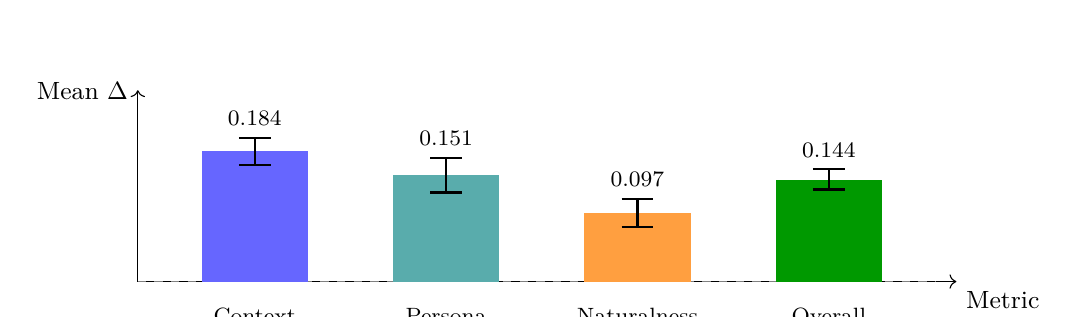
\begin{tikzpicture}[x=1.35cm,y=9.0cm]
\draw[->] (0.2,0) -- (7.9,0) node[below right] {\small Metric};
\draw[->] (0.2,0) -- (0.2,0.27) node[left] {\small Mean $\Delta$};
\draw[dashed,gray] (0.2,0) -- (7.7,0);

\fill[blue!60] (0.8,0) rectangle (1.8,0.1843);
\fill[teal!65] (2.6,0) rectangle (3.6,0.1509);
\fill[orange!75] (4.4,0) rectangle (5.4,0.0967);
\fill[green!60!black] (6.2,0) rectangle (7.2,0.1440);

\draw[thick] (1.3,0.1647) -- (1.3,0.2025);
\draw[thick] (1.15,0.1647) -- (1.45,0.1647);
\draw[thick] (1.15,0.2025) -- (1.45,0.2025);
\draw[thick] (3.1,0.1257) -- (3.1,0.1746);
\draw[thick] (2.95,0.1257) -- (3.25,0.1257);
\draw[thick] (2.95,0.1746) -- (3.25,0.1746);
\draw[thick] (4.9,0.0773) -- (4.9,0.1167);
\draw[thick] (4.75,0.0773) -- (5.05,0.0773);
\draw[thick] (4.75,0.1167) -- (5.05,0.1167);
\draw[thick] (6.7,0.1298) -- (6.7,0.1584);
\draw[thick] (6.55,0.1298) -- (6.85,0.1298);
\draw[thick] (6.55,0.1584) -- (6.85,0.1584);

\node[below=6pt,align=center] at (1.3,0) {\footnotesize Context};
\node[below=6pt,align=center] at (3.1,0) {\footnotesize Persona};
\node[below=6pt,align=center] at (4.9,0) {\footnotesize Naturalness};
\node[below=6pt,align=center] at (6.7,0) {\footnotesize Overall};
% Put labels above CI caps (not bar tops) and mask whiskers beneath labels.
\node[above,font=\footnotesize,fill=white,inner sep=1pt] at (1.3,0.2145) {0.184};
\node[above,font=\footnotesize,fill=white,inner sep=1pt] at (3.1,0.1866) {0.151};
\node[above,font=\footnotesize,fill=white,inner sep=1pt] at (4.9,0.1287) {0.097};
\node[above,font=\footnotesize,fill=white,inner sep=1pt] at (6.7,0.1704) {0.144};
\end{tikzpicture}
\caption{Paired mean-delta gains of controlled contextual generation over raw contextual generation, with 95\% CI whiskers.}
\label{fig:controlled_delta}
\end{figure}

Against phi3:mini no-context and phi3:latest no-context baselines, the controlled arm shows positive overall-quality deltas in both cross-condition comparisons. As summarized in Table~\ref{tab:baseline_comparison}, \(\Delta OQ\) is +0.1448 and +0.1475, both with strictly positive paired-bootstrap intervals.

\begin{table}[t]
\centering
\caption{Cross-condition \(OQ\) comparison: controlled contextual arm versus external no-context baselines under matched protocols.}
\label{tab:baseline_comparison}
\begingroup
\footnotesize
\setlength{\tabcolsep}{4pt}
\resizebox{\textwidth}{!}{%
\begin{tabular}{lcccc}
\toprule
Baseline & \(\Delta OQ\) & 95\% CI (\(\Delta OQ\)) & One-sided \(p\) & Holm-adjusted one-sided \(p\) (family size \(=2\)) \\
\midrule
phi3:mini & +0.1448 & [0.1314, 0.1571] & \(<1/\BootstrapSamples\) & \(<2/\BootstrapSamples\) \\
phi3:latest & +0.1475 & [0.1356, 0.1591] & \(<1/\BootstrapSamples\) & \(<2/\BootstrapSamples\) \\
\bottomrule
\end{tabular}}
\endgroup
\end{table}
Table~\ref{tab:chapter2_positioning} is a scoped qualitative synthesis under the report's stated criteria and search protocol, not a formal exhaustive ranking of the full literature.

Both paired-bootstrap intervals are strictly positive at the lower bound, confirming that the external-baseline overall-quality deltas are not borderline effects under the fixed-scenario protocol. Holm-adjusted one-sided \(p\)-value bounds remain below the finite-sample reporting floor for this two-comparison \(OQ\) family \cite{Holm1979}. Because these are cross-condition contrasts (contextual controlled vs no-context baselines), they support system-level gap reporting but do not identify isolated causal contribution of any single architectural component.

The remaining non-superior metrics are concentrated in lexical-diversity style indicators, not in grounding or consistency metrics. This pattern indicates a common control trade-off: stronger factual and persona anchoring may reduce stylistic entropy. In deployment settings where role consistency and state alignment are prioritized, this trade-off is usually acceptable.

Distinct-1 is lower for controlled generation than external baselines in current runs, indicating that stronger grounding can reduce lexical novelty in this setup. This is discussed as a design trade-off, not hidden.

To separate statistical from practical significance, the observed gains are interpreted against deployment objectives rather than significance alone. In this setting, the largest absolute improvements occur on context and persona metrics, which directly correspond to gameplay consistency requirements; therefore, these improvements are treated as operationally meaningful even when lexical-diversity indicators move in the opposite direction.

\subsection{Human evaluation and inter-rater agreement}
The human-evaluation report contains 324 ratings. Mean pairwise kappa across core metrics is 0.5329. Descriptive soft preference rates are 0.7315 against phi3:mini and 0.6806 against phi3:latest. Arm-level normalized overall quality means are 0.8037 for the controlled arm, 0.6944 for phi3:mini, and 0.7278 for phi3:latest.

The agreement profile (\(\kappa=0.5329\)) is consistent with moderate-to-substantial inter-rater reliability in subjective text assessment under commonly used interpretation ranges \cite{Landis1977KappaScale}. Preference outcomes are directionally aligned with automatic metrics, but because the campaign includes three raters and 324 ratings, this is treated as corroborative pilot-scale evidence rather than definitive standalone proof. In this report, soft preference rates are reported descriptively only; no confirmatory hypothesis tests, confidence-interval claims, or population-level preference inferences are drawn from these rates. A prospective power-based assignment plan for an expanded campaign is included in the human-evaluation package, but the larger follow-up ratings are not yet completed.

\subsection{Serving and retrieval performance trade-offs}

From the serving summary and delta reports, TTFT mean is 542.62 ms for the candidate model versus 273.86 ms for the baseline, total time mean is 3601.54 ms versus 3138.41 ms, and token throughput is 18.45 tokens/s versus 18.86 tokens/s. Serving-efficiency superiority is therefore not demonstrated.

This negative result is retained deliberately. The controlled architecture improves quality and robustness but incurs additional latency due to retrieval, guard scoring, and post-generation control. For production adoption, this implies a tunable frontier rather than a single dominant operating point.

On the retrieval axis, BM25 achieves Hit@5 = 1.0000, MRR = 0.8500, and nDCG@5 = 0.8893. Keyword-overlap retrieval reaches 0.9000, 0.8333, and 0.8500 on the same metrics; random retrieval gives 0.4000, 0.1650, and 0.2204; and the reranker method reports 0.9000, 0.8000, and 0.8262.

BM25 remains strongest on the current core label set, while the reranker is competitive and materially higher than random retrieval on observed point metrics. Because no formal hypothesis test was run for retrieval-method differences in this table, these contrasts should be read as descriptive effect magnitudes rather than inferential significance claims. This indicates that query-distribution effects matter: wider labeled sets are needed before asserting universal reranker superiority.

At training-stage granularity, the hard-negative reranker stage uses 3360 pairs (2856 train, 504 eval) and reports pair-accuracy 0.9563 with 95\% CI [0.9365, 0.9742].

Under adversarial stress, both poisoned and trust-spoofed test sets (100 scenarios each) show baseline ASR = 1.0000, guarded ASR = 0.0000, and relative reduction = 1.0000, with confidence intervals included in artifact reports. For the guarded condition with 0/100 observed successes per set, the exact 95\% upper bound on ASR is \(1-0.05^{1/100}\approx 0.0295\) for each set; pooled across both guarded sets (0/200), the exact 95\% upper bound is \(1-0.05^{1/200}\approx 0.0149\).

From a deployment perspective, this is one of the most consequential findings in this benchmark. The guard layer does not merely reduce average error; no successful follow-through was observed on the tested adversarial injections under the evaluated protocol (with exact 95\% upper ASR bound 0.0295 per 100-case stress set). The claim is intentionally restricted to the tested attack families and sample size, not generalized to all adversarial regimes.

\subsection{UE5 operational metrics and behavior-state effects}
To complement text-quality outcomes, operational runtime metrics are reported for the same 112-scenario controlled arm used in the main benchmark summary. Metrics follow the Chapter 3 definitions and are computed from turn-level operational traces (\texttt{response\_fallback}, \texttt{rewrite\_attempts}, and repair markers). The hard timeout criterion is request-level timeout failure in the benchmark harness (\texttt{timeout\_s}=180). In this section, retry rate denotes controller intervention frequency (turns with at least one rewrite/regeneration attempt), not hard request failure.

\begin{table}[t]
\centering
\caption{UE5-relevant operational runtime metrics (controlled arm, \(N=112\)).}
\label{tab:ue5_operational_metrics}
\begingroup
\footnotesize
\setlength{\tabcolsep}{4pt}
\begin{tabular}{p{0.31\textwidth}p{0.23\textwidth}p{0.17\textwidth}p{0.22\textwidth}}
\toprule
Metric & Criterion & Value & Exact 95\% CI \\
\midrule
Timeout rate & timeout failures / 112 turns & 0.0000 (0/112) & [0.0000, 0.0324] \\
Error rate & failed requests / 112 turns & 0.0000 (0/112) & [0.0000, 0.0324] \\
Fallback rate & fallback outputs / 112 turns & 0.0089 (1/112) & [0.0002, 0.0487] \\
First-pass acceptance rate & accepted without rewrite / 112 turns & 0.3750 (42/112) & [0.2853, 0.4715] \\
Rewrite-attempt rate & turns with rewrite attempts \(>0\) & 0.1071 (12/112) & [0.0566, 0.1797] \\
Retry rate & turns with retries \(>0\) & 0.1071 (12/112) & [0.0566, 0.1797] \\
Rewrite-failure rate & rewrite failure / 112 turns & 0.0000 (0/112) & [0.0000, 0.0324] \\
\bottomrule
\end{tabular}
\endgroup
\end{table}

The results show zero hard timeout failures and low hard-intervention burden under the current control profile. Table~\ref{tab:ue5_operational_metrics} indicates that fallback and retry are both low (0.0089 and 0.1071), while first-pass acceptance remains below half of turns (0.3750); this means stability is achieved largely through non-retry control paths (e.g., structured repair) rather than repeated regeneration. This pattern is consistent with the latency trade-off already observed in serving benchmarks: admissibility constraints improve grounding robustness while adding per-turn control overhead.

Because the system is behavior-conditioned in UE5, operational variation by NPC behavior state is also reported.

\begin{table}[t]
\centering
\caption{Behavior-state-conditioned operational impact (controlled arm).}
\label{tab:ue5_state_operational}
\begingroup
\footnotesize
\setlength{\tabcolsep}{4pt}
\begin{tabular}{lcccc}
\toprule
Behavior state & \(n\) & Fallback rate & Rewrite-attempt rate & Mean overall quality \\
\midrule
Assisting & 23 & 0.0000 & 0.2174 & 0.3645 \\
Detained & 3 & 0.0000 & 1.0000 & 0.3063 \\
Forging & 5 & 0.0000 & 0.0000 & 0.4075 \\
Guarding & 4 & 0.0000 & 0.0000 & 0.4385 \\
Investigating & 11 & 0.0000 & 0.0000 & 0.3908 \\
Negotiating & 8 & 0.1250 & 0.2500 & 0.3788 \\
Observing & 24 & 0.0000 & 0.0833 & 0.3858 \\
Patrolling & 8 & 0.0000 & 0.0000 & 0.4045 \\
Researching & 11 & 0.0000 & 0.0000 & 0.3734 \\
Ritual preparation & 5 & 0.0000 & 0.0000 & 0.3494 \\
Trading & 3 & 0.0000 & 0.0000 & 0.3829 \\
Treating patient & 7 & 0.0000 & 0.0000 & 0.3950 \\
\bottomrule
\end{tabular}
\endgroup
\end{table}

The state-conditioned pattern indicates that operational stability is not uniform across gameplay modes. Guarding and patrolling retain comparatively higher mean overall quality, while detained and negotiating states carry the heaviest rewrite pressure. This supports a UE5 tuning policy in which control thresholds are tuned by behavior-state family rather than globally before production deployment decisions are made.

\subsection{Operating-point diagnostics: quality, latency, and intervention coupling}
To convert the above findings into deployment-oriented decision signals, three derived diagnostics are reported using observed benchmark values. First, quality throughput is defined as:
\begin{equation}
\mathrm{QTPS}=\frac{OQ}{T_{total}^{(s)}},
\end{equation}
where \(T_{total}^{(s)}\) is total response time in seconds. Second, intervention burden is summarized as:
\begin{equation}
\mathrm{IBI}=1-\mathrm{FirstPassAcceptRate}.
\end{equation}
Third, recovery dependence is summarized by:
\begin{equation}
\mathrm{RDI}=\frac{\mathrm{RetryRate}}{\max(\mathrm{FirstPassAcceptRate},\epsilon)},
\end{equation}
with \(\epsilon=10^{-6}\) for numerical safety.

\begin{table}[t]
\centering
\caption{Derived operating-point diagnostics from reported benchmark values.}
\label{tab:operating_point_diagnostics}
\begingroup
\footnotesize
\setlength{\tabcolsep}{4pt}
\begin{tabular}{p{0.41\textwidth}p{0.22\textwidth}p{0.30\textwidth}}
\toprule
Diagnostic & Value & Interpretation \\
\midrule
\(\Delta OQ\) vs phi3:mini no-context & \(+0.1448\) & Positive cross-condition quality gap \\
Total-latency overhead vs phi3:mini & \(+14.76\%\) & Candidate is slower at this operating point \\
QTPS (candidate) & \(0.1058\) & \(0.3811/3.60154\) quality units per second \\
QTPS (phi3:mini) & \(0.0753\) & \(0.2363/3.13841\) quality units per second \\
IBI (candidate) & \(0.6250\) & First-pass acceptance remains limited \\
RDI (candidate) & \(0.29\) & Retry burden is low relative to accepted first-pass turns \\
Fallback-to-first-pass ratio (candidate) & \(0.02\) & \(1/42\), fallback is rare at this operating point \\
\bottomrule
\end{tabular}
\endgroup
\end{table}

Table~\ref{tab:operating_point_diagnostics} reinforces the bounded interpretation used throughout this report: quality improvements are observable, but they are currently obtained with high control intervention. The principal engineering target for the next cycle is therefore not additional quality-only gain, but reducing intervention burden at fixed safety and quality floors using the state-conditioned calibration policy in Section 3.4.

\subsection{Component-level ablation results}

To interpret the ablation results rigorously, each reported component effect is defined as a conditional mean difference on metric \(m\):
\begin{equation}
\hat{\delta}_{m,c}=\mathbb{E}[m\mid c=1]-\mathbb{E}[m\mid c=0],
\end{equation}
where \(c\in\{\text{context},\text{guard},\text{control}\}\). In this run, the logged ablation design supports direct main-contrast estimates only; full interaction estimation was prespecified but is not reported because full factorial switch-off arms were not available for every component pair.

\begin{algorithm}[H]
\caption{Main-contrast ablation effect estimation}
\begin{algorithmic}[1]
\Require scenario-level metric dataset \(\mathcal{D}_{abl}=\{(m_i,\mathbf{c}_i)\}_{i=1}^{N}\), component set \(\mathcal{C}\)
\Require bootstrap count \(B\)
\For{each metric \(m\)}
  \For{each component \(c\in\mathcal{C}\)}
    \State compute paired contrast \(\hat{\delta}_{m,c}=\mathbb{E}[m\mid c{=}1]-\mathbb{E}[m\mid c{=}0]\)
    \State bootstrap paired scenarios \(B\) times to obtain \(CI_{95}(\hat{\delta}_{m,c})\) and one-sided \(p(\hat{\delta}_{m,c}\le0)\)
  \EndFor
\EndFor
\State return main-contrast summary tables with uncertainty
\end{algorithmic}
\end{algorithm}

Table~\ref{tab:ablation_response_control} reports the observed response-control main contrast with uncertainty estimates, while Tables~\ref{tab:ablation_retrieval} and~\ref{tab:ablation_serving} report retrieval and serving ablations. This layout makes each reported architectural trade-off numerically explicit rather than summary-only.

\begin{table}[t]
\centering
\caption{Response-control ablation (controlled contextual vs. raw contextual).}
\label{tab:ablation_response_control}
\begingroup
\footnotesize
\setlength{\tabcolsep}{4pt}
\begin{tabular}{lccc}
\toprule
Metric & Mean \(\Delta\) & 95\% CI & \(p(\Delta\le0)\) \\
\midrule
Context relevance & +0.1843 & [0.1647, 0.2025] & \(<1/\BootstrapSamples\) \\
Persona consistency & +0.1509 & [0.1257, 0.1746] & \(<1/\BootstrapSamples\) \\
Naturalness & +0.0967 & [0.0773, 0.1167] & \(<1/\BootstrapSamples\) \\
Overall quality & +0.1440 & [0.1298, 0.1584] & \(<1/\BootstrapSamples\) \\
BERTScore F1 & +0.0205 & [0.0088, 0.0327] & \(<1/\BootstrapSamples\) \\
Distinct-1 & -0.0011 & [-0.0097, 0.0068] & 0.5963 \\
\bottomrule
\end{tabular}
\endgroup
\end{table}

In Table~\ref{tab:ablation_response_control}, inferential interpretation remains two-tiered as defined in Chapter 3: \(CR\), \(PC\), \(N\), and \(OQ\) are confirmatory core metrics, while BERTScore F1 and Distinct-1 are supportive diagnostics reported without additional multiplicity adjustment in this table.
Within the confirmatory four-metric family (\(CR,PC,N,OQ\)), Holm-adjusted one-sided \(p\)-value bounds remain below \(4/\BootstrapSamples=0.0008\), so the core conclusions are unchanged under this family-wise correction \cite{Holm1979}.

\begin{table}[t]
\centering
\caption{Retrieval-method ablation deltas relative to BM25 (higher is better).}
\label{tab:ablation_retrieval}
\begingroup
\footnotesize
\setlength{\tabcolsep}{4pt}
\begin{tabular}{lccc}
\toprule
Method & Hit@5 \(\Delta\) & MRR \(\Delta\) & nDCG@5 \(\Delta\) \\
\midrule
Keyword overlap & -0.1000 & -0.0167 & -0.0393 \\
Random & -0.6000 & -0.6850 & -0.6688 \\
Reranker & -0.1000 & -0.0500 & -0.0631 \\
\bottomrule
\end{tabular}
\endgroup
\end{table}

\begin{table}[t]
\centering
\caption{Serving ablation (candidate vs. baseline phi3:mini).}
\label{tab:ablation_serving}
\begingroup
\footnotesize
\setlength{\tabcolsep}{4pt}
\begin{tabular}{lcccc}
\toprule
Metric & Candidate & Baseline & \(\Delta\) & Better? \\
\midrule
TTFT (ms) & 542.62 & 273.86 & +268.76 & No \\
Total time (ms) & 3601.54 & 3138.41 & +463.13 & No \\
Tokens/s & 18.45 & 18.86 & -0.41 & No \\
\bottomrule
\end{tabular}
\endgroup
\end{table}

Under this framework, the reported response-control main contrast is positive on the core quality axes. Table~\ref{tab:ablation_response_control} shows that all core quality metrics have strictly positive confidence intervals and one-sided \(p\)-values at the reporting floor, while Distinct-1 is not significant at conventional levels; this supports a controlled-quality gain with a mild style-diversity trade-off. The outcome is consistent with the design hypothesis that retrieval improves available evidence but does not itself enforce admissibility constraints on generated text. In practice, reducing response control increases context omissions and persona drift even when retrieval quality is unchanged, indicating that evidence quality and output admissibility are separable control problems.

Under the current core retrieval set, BM25 remains strongest. Table~\ref{tab:ablation_retrieval} quantifies this directly, with all tested alternatives showing negative deltas relative to BM25 on Hit@5, MRR, and nDCG@5. This does not invalidate reranker training quality; instead, it indicates that method-level superiority is query-distribution dependent and should be evaluated on wider labeled sets with broader lexical and semantic variation. The architecture uses hybrid retrieval with guard-aware penalties because each component addresses a different failure mode: sparse retrieval preserves exact-key matching for inventory and quest references, dense retrieval improves semantic recall for paraphrased user input, and guard penalties are designed to reduce susceptibility to poisoned or trust-spoofed evidence. This design choice is aligned with the failure modes highlighted by recent adversarial-retrieval literature \cite{Zou2025PoisonedRAG,Chaturvedi2025AIP}. In this report, retrieval-table ablations quantify relevance trade-offs, while guard safety effects are evidenced by the dedicated adversarial stress tests; interpreted jointly, they indicate a safety-oriented operating trade-off that can reduce recall on ambiguous queries.

Latency and throughput deltas remain unfavorable for the candidate at the current quality configuration, as shown in Table~\ref{tab:ablation_serving}. This pattern is expected from the architecture: guard scoring and response-control evaluation add deterministic overhead, and retrieval-conditioned prompts increase prefill and decoding work relative to no-context baselines. A useful comparison strategy is equal-quality frontier analysis, where each system is evaluated at the minimum latency required to satisfy a fixed quality target. This avoids misleading conclusions in which a faster model is favored only because it operates at a lower quality point. Taken together, the ablations support bounded conclusions only on observed contrasts: response-control main contrast is positive for quality in this design, evaluated stress-test outcomes improve under guard-enabled settings, and serving efficiency remains the principal unresolved bottleneck.

To keep chapter-level interpretation auditable, Table~\ref{tab:claim_evidence_map} consolidates the primary claims against their direct evidence and support status under the current protocol.

\begin{table}[t]
\centering
\caption{Claim-to-evidence synthesis for principal findings.}
\label{tab:claim_evidence_map}
\begingroup
\footnotesize
\setlength{\tabcolsep}{4pt}
\begin{tabular}{p{0.30\textwidth}p{0.43\textwidth}p{0.20\textwidth}}
\toprule
Claim & Direct evidence in this report & Support status \\
\midrule
Controlled contextual inference improves core dialogue quality over raw contextual inference & Table~\ref{tab:ablation_response_control}, Fig.~\ref{fig:controlled_delta}: positive \(\Delta CR\), \(\Delta PC\), \(\Delta N\), \(\Delta OQ\) with strictly positive 95\% CIs & Supported under fixed-scenario protocol \\
Controlled contextual setting shows a cross-condition quality advantage over external no-context baselines & Table~\ref{tab:baseline_comparison}: positive \(\Delta OQ\) with strictly positive CI lower bounds in both comparisons and Holm-adjusted one-sided \(p\) bounds for the two-comparison \(OQ\) family & Supported as cross-condition gap (not isolated component causality) \\
Guarded retrieval improves adversarial outcomes in evaluated stress sets & Security results: ASR reduced from 1.0000 to 0.0000 on both poisoned and trust-spoofed stress sets (\(n=100\) each) & Supported for tested attack families and sample size \\
Architecture is faster than lightweight baselines at current operating point & Table~\ref{tab:ablation_serving}: TTFT and total latency higher; throughput slightly lower than baseline & Not supported \\
Low-intervention runtime behavior at the current operating point & Table~\ref{tab:ue5_operational_metrics}: fallback 0.0089, retry 0.1071, first-pass acceptance 0.3750 & Partially supported (fallback/retry low, first-pass still limited) \\
\bottomrule
\end{tabular}
\endgroup
\end{table}

\subsection{Threats to validity and interpretive boundaries}
Internal validity is influenced by threshold selection in response control and guard scoring, even when pipeline automation reduces manual evaluation bias. This risk is mitigated through explicit artifact release, ablation reporting, Python-C++ parity checks, and prompt-template controls that enforce consistent field ordering and key normalization between benchmark and runtime paths. Another internal threat is evaluator-mediated bias in automatic quality judgments. Although the current protocol combines automatic and human ratings, judge-style evaluation frameworks can still carry position and verbosity biases \cite{Zheng2023MTBench,Wang2024Judge,Dubois2024AlpacaEval}; consequently, interpretation emphasizes convergent trends across independent metrics rather than a single score family.

External validity remains limited by label coverage and genre coverage. The core retrieval label set is still relatively small, so retrieval-superiority conclusions are intentionally constrained until wider-domain labels are integrated. Generalization to other game genres is also uncertain, because narrative role-play settings differ from sandbox or competitive multiplayer contexts where brevity and tempo can dominate response quality requirements. In addition, scenario-dependence diagnostics show partial template clustering (\(71/112\) unique template signatures, effective sample size by template signature \(\approx 56\), and source-level effective sample size \(=8\)); inferential strength should therefore be interpreted conservatively outside this benchmark design. This limitation is consistent with the broader LLM-in-games literature, which reports promising interaction gains while still facing transfer and deployment-friction challenges across platforms and play styles \cite{Gallotta2024Survey,Sweetser2024Scoping,Rao2024Minecraft}.

Construct validity is constrained by the multi-dimensional nature of dialogue quality. No single metric captures ``good NPC dialogue,'' so the study uses a bundle of context, persona, naturalness, overall quality, retrieval, serving, and security metrics with human preference checks. Even under this design, construct drift can occur when raters interpret naturalness differently; the protocol addresses this by providing rubric definitions with worked examples during rater onboarding. In addition, retrieval-robustness constructs can be sensitive to attack design, and different adversarial families may produce different failure profiles \cite{Zou2025PoisonedRAG,Chaturvedi2025AIP}.

Reproducibility validity is affected by runtime drift in model revisions, serving backends, and library stacks. To reduce ambiguity, the pipeline records run metadata and executable manifests. A related risk is metric coupling, where improvements in one axis suppress another; this is handled by reporting both gains and trade-offs instead of collapsing results into a single opaque score. This reporting choice follows recent recommendations in evaluation practice that discourage one-number claims for complex interactive systems \cite{Liang2023HELM,Wang2024Judge,Dubois2024AlpacaEval}.

\subsection{Comparison with prior work and practical implications}
The central finding is not that one model is universally superior. Under this protocol, integrating context extraction, guard-aware retrieval, and response control improves context and persona quality relative to the raw contextual arm, while also improving outcomes in the tested adversarial sets. Relative to prior work focused primarily on interaction quality \cite{Park2023GenerativeAgents} or retrieval-aware generation quality \cite{Asai2024SelfRAG,Edge2024GraphRAG}, the contribution here is the explicit integration of these components with runtime admissibility control and adversarial evaluation in one in-engine pipeline.

This distinction matters for scientific reporting. Many studies demonstrate promising prompts but under-specify runtime control logic, which weakens replicability and deployment relevance. In this report, runtime and evaluation paths are intentionally coupled, and claims are bounded by explicit criteria. The observed pattern is consistent across sections: response-control contrasts are positive on core quality metrics, guard-enabled settings improve results in tested adversarial conditions, and systems efficiency remains the main bottleneck. These are protocol-specific findings, not a full causal decomposition, and therefore do not imply automatic latency gains.
Accordingly, the comparative-positioning statement in this report is scoped to the reviewed literature and measured protocol, and is not presented as a universal ``first-in-field'' claim.

From an engineering perspective, the current configuration should still be treated as a quality-and-robustness prototype rather than a final production operating point: hard interventions are now low, but first-pass acceptance remains limited and serving speed remains slower than lightweight baselines. If throughput is the primary objective, lighter serving configurations still hold an advantage, including settings optimized around speculative decoding and memory-efficient serving stacks \cite{Leviathan2022SpecDec,Kwon2023vLLM}. The practical implication is to choose deployment points on an explicit quality-latency frontier rather than on raw speed alone.

An additional practical implication is workflow design. Teams can adopt the architecture incrementally: first introduce state serialization and evaluation harnesses, then add guarded retrieval, and finally add response control with parity tests. This staged integration reduces adoption risk for existing production pipelines while preserving traceability of where specific gains originate.

The broader significance is interdisciplinary. The system sits at the intersection of game AI, natural language generation, retrieval security, and human-centered evaluation. As a result, progress depends on coordinated advances in all four areas rather than isolated gains in any single subfield. This interdisciplinary framing also motivates the report's evaluation breadth: narrative quality, robustness, and serving behavior are treated as jointly necessary for practical deployment.

\section{Conclusions, implications, and future directions}
This chapter synthesizes the findings into bounded scientific conclusions and deployment implications. It distinguishes supported claims from unresolved limitations and then outlines the most consequential next steps for both research and practice.
\subsection{Ethical and policy implications for NPC deployment}
The architecture is designed for interactive entertainment, but its risk profile is not limited to content quality. Role-grounded generation can amplify stereotypes or exclusionary language if persona definitions or retrieval corpora are biased, and retrieval pipelines can be exploited through adversarial artifacts that appear authoritative. These concerns are consistent with broader analyses of social and safety risks in large language models \cite{Bender2021Parrots,Weidinger2022Taxonomy}. In response, the study includes explicit adversarial evaluation, response-level admissibility checks, and transparent reporting of both gains and failure trade-offs.

Data governance and user trust present a second ethical axis. Narrative-game interactions can contain sensitive player behavior signals, so context serialization and logging must minimize unnecessary retention and avoid exposing private state attributes. Although this report focuses on algorithmic performance rather than legal compliance design, the reporting protocol is structured to support external audit by making metric procedures, confidence intervals, and stress-test outcomes inspectable. This is particularly important where systems can be manipulated through prompt-level and retrieval-level attacks \cite{Zou2025PoisonedRAG,Chaturvedi2025AIP}.

Finally, responsible deployment requires clarity about what the system does not guarantee. The current evidence supports improvements in grounded quality and robustness under the evaluated benchmark, but does not establish universal safety or universal generalization. For this reason, claims are bounded to measured conditions, and negative findings are retained. This policy follows the same principle underlying alignment and constitutional approaches: safety mechanisms should be treated as operational constraints that require continuous measurement, not one-time guarantees \cite{Bai2022Constitutional}.

From a management perspective, a staged readiness policy is recommended: first reduce intervention burden (fallback/retry) through threshold and prompt-policy retuning in controlled pilots, then evaluate live telemetry for stability, and only then consider broader deployment. This sequencing aligns operational risk control with measured evidence and prevents premature optimization for stylistic variability at the expense of consistency and safety.

\subsection{Principal findings and bounded claims}
This paper presents a full system and evaluation framework for dynamic game-state-informed NPC dialogue in narrative games. The proposed pipeline demonstrates consistent improvements in context relevance, persona consistency, and overall dialogue quality over the raw contextual arm, together with favorable adversarial outcomes in the evaluated poisoning/trust-spoof stress tests.

The study yields a conditional conclusion rather than a universal one: the architecture is advantageous when grounded quality and robustness are primary objectives, and less advantageous when latency is the dominant objective.

\subsection{Study limitations}
Five limitations are central. First, operational reliability in UE5 is improved but still incomplete: fallback and retry are low (0.0089 and 0.1071), yet first-pass acceptance remains 0.3750 (Table~\ref{tab:ue5_operational_metrics}), indicating continued dependence on control-layer repair paths at runtime. Second, cross-baseline superiority statements are confounded by contextual-condition differences and therefore should be read as system-level gaps rather than isolated architectural effects. Third, exploratory multi-metric comparisons are reported without family-wise multiplicity adjustment, and UE5 operational diagnostics are estimated from one benchmark run with exact binomial intervals only, not from repeated-run mixed-effects modeling; these operational estimates are therefore descriptive rather than confirmatory. Fourth, human-evaluation sampling is pilot-scale; a prospective power-based assignment plan exists for a larger campaign, but expanded ratings are not yet completed. Fifth, generalization beyond narrative-role-play conditions remains unverified for faster interaction genres with stricter response-time constraints, and scenario-dependence remains non-negligible (effective sample size by template signature \(\approx 56\), source-level effective sample size \(=8\)). These limitations keep the conclusion deliberately conditional rather than universal.

\subsection{Future research agenda}
Future work should focus on five concrete upgrades: state-conditioned control-threshold calibration to reduce fallback/retry burden under fixed safety caps, quality-preserving acceleration for lower-intervention runtime operation, broader retrieval labels and lower-dependence scenario expansion for stronger external validity, repeated UE5 operational runs with mixed-effects uncertainty modeling for stability claims, and completion of the power-planned larger human-evaluation campaign with broader rater diversity. These steps are necessary to determine whether the observed gains generalize under broader workloads and stricter real-time constraints.

\section*{Artifact and reproducibility statement}
All quantitative conclusions in this report are grounded in versioned supplementary artifact bundles, including run manifests, metric summaries, confidence-interval reports, raw benchmark traces, and analysis scripts. The package is structured to support independent verification of every reported numerical result.

\appendix
\titleformat{\section}{\bfseries\fontsize{15}{20}\selectfont}{Appendix \thesection:}{0.6em}{}

\section{Reproducibility protocols and extended methods}
This appendix section consolidates procedural details required for independent reproduction of the reported results. It expands implementation-level decisions, protocol settings, and audit conventions that are summarized in the main chapters.
\subsection{Scenario taxonomy}
The 112-scenario set is generated to cover heterogeneity in archetype, conflict type, location type, and behavior state. Archetypes include guard, scholar, merchant, healer, outlaw, and ritual specialist roles. Conflict categories include denial, negotiation, urgency, deception attempt, and memory conflict. Location categories include city, shrine, wilderness, naval, law hall, and market contexts. Behavior states include patrol, investigation, combat-ready, idle social, quest handoff, and recovery modes.

The design goal is to reduce overfitting to one style of prompt and create meaningful variance for context and persona checks. Each scenario includes expected context keys and role cues to support metric computation and qualitative inspection.

\subsection{Prompt and context serialization specification}
Prompt layout is deterministic with bounded sections: persona block, context block, retrieval evidence block, and user utterance. Context keys are normalized to reduce alias ambiguity. Free-form key generation is avoided at runtime; only predefined keys are emitted by context extraction modules. This design simplifies parser logic and lowers failure probability in downstream post-processing.

\subsection{Response-control specification}
The response controller evaluates candidate outputs through a sequence of structural and semantic checks that include prohibited-pattern filtering, context-key alignment scoring, persona-style consistency assessment, and minimal coherence and length checks before fallback decisions are applied. The C++ implementation mirrors Python-side behavior to prevent benchmark-vs-runtime divergence. For factual-stability diagnostics, sampled self-consistency signals are also monitored as a secondary alert channel, following the black-box consistency principle demonstrated in hallucination-detection work such as SelfCheckGPT \cite{Manakul2023SelfCheckGPT}.

\subsection{Adversarial retrieval protocol}
Adversarial sets include poison documents and trust-spoofed variants that imitate metadata authority. Baseline is retrieval without guard penalty. Guarded condition applies risk/trust penalties and directive checks before final ranking. Attack success is measured by whether the system follows poisoned directives. This binary framing is intentionally conservative.

\subsection{Human evaluation protocol}
The campaign uses three independent raters and shared overlap to estimate inter-rater agreement. Metrics are normalized to [0,1] and include context relevance, persona consistency, naturalness, and overall quality. Pairwise kappa is reported per metric and aggregated by mean.

\subsection{Compute and runtime environment}
Serving and evaluation are executed with local inference endpoints and recorded host metadata. The pipeline captures model IDs, prompts, and configuration parameters (temperature, max tokens) to support reruns. CMake-based C++ builds and Python orchestration are executed through reproducible command manifests.
For deterministic report builds, the document is compiled from the \texttt{docs/} directory using XeLaTeX only (\texttt{xelatex IEEE\_FULL\_PAPER.tex} run at least twice, and a third pass after major label or citation edits). Mixed working directories or pdfLaTeX runs can produce stale auxiliary-reference warnings in the presence of Unicode cover pages.

\subsection{Literature-screening protocol for comparative positioning}
The comparative-positioning statement in Chapter 2 is based on a targeted narrative search, not on a formal PRISMA-style systematic review \cite{Page2021PRISMA2020}. Search sources were IEEE Xplore, ACM Digital Library, ACL Anthology, and arXiv over January 2020--February 2026. Query families included combinations of: ``NPC dialogue'' OR ``LLM game agents''; ``game-state grounding''; ``retrieval-augmented generation'' AND (``poisoning'' OR ``prompt injection'' OR ``trust spoofing''); and ``runtime evaluation'' OR ``in-engine benchmark''. Reproducible query templates were defined as text fields over title/abstract/keywords, including: \(Q_1\): (``NPC dialogue'' OR ``non-player character dialogue'') AND (``large language model'' OR LLM) AND (game OR ``narrative game''); \(Q_2\): (``game state'' OR ``world state'') AND (grounding OR context) AND (dialogue OR interaction); \(Q_3\): (``retrieval-augmented generation'' OR RAG) AND (poisoning OR ``prompt injection'' OR ``indirect prompt injection'' OR ``trust spoofing''); \(Q_4\): (``runtime'' OR ``in-engine'') AND (evaluation OR benchmark) AND (agent OR dialogue).

Inclusion criteria were: direct relevance to interactive game/NPC dialogue or closely adjacent LLM-agent runtime control, explicit method description, and empirical evaluation details sufficient for comparative positioning. Exclusion criteria were: purely conceptual opinion pieces without empirical methods, non-game domains without transferable runtime-control mechanisms, and non-English records lacking technical detail required for method-level comparison.

Citation formatting prioritizes archival venue metadata and DOI when verifiably available. Preprint-only records are retained when no archival version could be confirmed at report freeze, and these are explicitly presented as preprints rather than evidence-equivalent substitutes for peer-reviewed venues. A final venue audit was run on March 4, 2026 against DBLP and Crossref; entries that remain in arXiv/CoRR form did not have verified archival venue metadata at that date.

Because the process was targeted and hypothesis-driven, it supports scoped comparative positioning but does not guarantee exhaustive field coverage. In addition, PRISMA-style screening flow counts were not maintained because the review was not executed as a formal systematic-review protocol. For this reason, Chapter 2 does not claim ``first-in-field'' novelty; it reports bounded comparative evidence under explicit scope and protocol constraints.

\section{Extended interpretation and comparative notes}
This appendix section provides interpretive extensions that would otherwise interrupt the main argument flow. It retains comparative nuance, additional limitations context, and design reflections while preserving claim discipline from the core chapters.
\subsection{Comparative-scope limitations}
This work compares against external baselines under identical prompts and datasets, which is appropriate for engineering benchmarking but not equivalent to full protocol replication of each cited paper. Conclusions in this report are therefore constrained to axes directly measured in the recorded benchmark artifacts.

\subsection{Future work plan}
The immediate roadmap includes decode-path acceleration with quality-parity checks, expansion of the official retrieval label set, larger mixed human-subject and expert-rater studies, explicit equal-quality serving-frontier reporting, and uncertainty-aware calibration of response-control thresholds.

\subsection{Detailed reproducibility report}
This section is intentionally detailed to serve two goals: first, to document full implementation logic for independent reproduction; second, to provide the depth typically expected in long-format engineering papers where the contribution combines system design, evaluation protocol, and deployment constraints rather than a single model novelty. The text below is organized as procedural documentation in IEEE narrative style.

Methodological reporting is aligned with reproducibility-first practice: every benchmark run is linked to a manifest containing model identity, decoding configuration, scenario slice, and hash-stamped artifact outputs. The intent is to make each reported number traceable from report table to executable run state, consistent with recommendations from reproducibility initiatives in machine learning \cite{Pineau2021Reproducibility}.

Scenario construction follows a templated expansion approach. A base scenario definition contains archetype, locale, conflict objective, state variables, and success conditions. The generator expands each base by varying one or more dimensions while preserving semantic validity constraints. For example, if archetype is ``temple scholar,'' conflict variants can include misinformation injection, urgency override, contradictory memory challenge, and authority spoofing; however, item-trade conflict templates are disabled unless the scenario includes an economic context key.

Data validation occurs in three stages. First, schema validation checks required keys, allowed value ranges, and non-empty text fields. Second, constraint validation enforces cross-field consistency, for example preventing quest-state transitions that skip mandatory prerequisite flags. Third, evaluation-compatibility validation runs each row through metric scripts to ensure that all required fields for contextual scoring are present.

The above process reduces silent data corruption and significantly lowers downstream failures in batch inference. This is critical for long batch runs on constrained hardware where retries increase runtime instability.

Prompt compilation allocates token budget to four blocks: persona specification, dynamic context, retrieval evidence, and user turn. Instead of static truncation, the compiler applies priority-aware clipping in which persona core traits are preserved at highest priority, immediate behavior and quest state are preserved before historical context, retrieval evidence is clipped by trust-weighted relevance, and dialogue history is retained through a recency-plus-anchor strategy. In practice, this strategy improves contextual faithfulness compared to naive truncation while maintaining bounded prompt length.

Let \(r_i\) be base retrieval relevance and \(g_i\) be guard penalty:
\[
s_i = r_i - \lambda g_i,
\]
where \(g_i\) aggregates injection cue score, trust-spoof likelihood, and metadata inconsistency checks. Candidate documents are ranked by \(s_i\), not \(r_i\). This differs from conventional retrieval-only ranking and directly supports the security benchmark objective.

Given raw generation \(\hat{y}\), response control computes:
\[
F(\hat{y}) = w_c \phi_c + w_p \phi_p + w_n \phi_n - w_v \phi_v,
\]
where \(\phi_c\) is context consistency, \(\phi_p\) persona style, \(\phi_n\) naturalness proxy, and \(\phi_v\) violation risk. If \(F(\hat{y}) < \tau\), fallback policy triggers grounded safe response generation. Thresholds are tuned on development scenarios and then frozen for benchmark runs.

Large evaluations are executed in batch mode with run-state persistence. In each batch, the runner loads the next scenario slice, executes all arms under fixed generation settings, writes raw request and response logs immediately, updates the checkpoint manifest, and computes per-batch health metrics. If process interruption occurs, execution resumes from the last completed batch index. This design is necessary because long cloud notebook sessions can terminate unexpectedly.

Three safeguards are used: no synthetic NaN filling for missing arms, minimum arm success-rate checks before summary emission, and evidence-completeness criteria that block summary emission when required checks are absent. These controls are simple but effective at preventing accidental overstatement from incomplete runs.

\subsection{Supplementary comparative discussion}
Compared with generative-agent systems that prioritize social simulation and reflective memory loops \cite{Park2023GenerativeAgents}, the present architecture is narrower in behavioral scope but stronger in runtime instrumentation and inferential control. The intended contribution is therefore not broad social realism, but auditable state-grounded dialogue under engine constraints within a fixed benchmark protocol.

Relative to serving-efficiency literature, speculative decoding and optimized serving engines provide clear throughput advantages in many workloads \cite{Leviathan2022SpecDec,Kwon2023vLLM}. The current system does not outperform such baselines on latency or throughput, and this negative result is retained explicitly to separate quality and robustness improvements from systems-efficiency outcomes.

Relative to retrieval-grounded generation literature, modern retrieval-plus-critique and graph-augmented pipelines improve factual conditioning \cite{Asai2024SelfRAG,Edge2024GraphRAG,Fan2024RAGSurvey}, but adversarial evidence handling remains comparatively under-reported in game-specific pipelines. In this study, one notable observed gain is on the robustness axis, where guarded retrieval yields 0 observed attack-follow cases in the evaluated stress protocol (two tested families, \(n=100\) each), which should not be generalized beyond that scope.

Relative to alignment and preference-learning work \cite{Ouyang2022InstructGPT,Rafailov2023DPO,Bai2022Constitutional}, the design choice in this paper is to complement training-time alignment with runtime control. Response control is treated as a deterministic admissibility layer that can enforce context and persona constraints turn-by-turn, even when upstream generation confidence is unstable.

Finally, relative to evaluation practice based only on overlap-style scoring, this report adopts a broader evidence model combining context and persona metrics, inferential significance testing, preference outcomes, and agreement statistics \cite{Zhang2020BERTScore,Zheng2023MTBench,Wang2024Judge,Dubois2024AlpacaEval,Cohen1960Kappa}. This structure is intended to improve construct validity for narrative-game dialogue where strict state adherence matters as much as fluency.

\subsection{Failure taxonomy}
Failure analysis uses five high-level classes: context omission, where the response ignores a critical state variable; persona drift, where response style diverges from the NPC role profile; instruction hijack, where malicious or irrelevant retrieval cues redirect behavior; temporal inconsistency, where the response contradicts recent dialogue memory; and over-constrained language, where control pressure yields rigid but less natural text.

Each class is tracked with examples during validation. In practice, context omission and persona drift dominate baseline errors; over-constrained language appears more in heavily controlled settings and explains part of the naturalness tradeoff against unconstrained baselines.

Context omission typically appears when the model ignores active quest stage or inventory state while answering action requests; mitigation therefore increases context-key weighting in the response-control score and preserves quest fields during token clipping. Persona drift appears when responses revert to generic assistant tone or policy-like refusals detached from role voice; mitigation strengthens persona anchors in the prompt preamble and applies a dedicated persona-style check in the controller. Retrieval hijack appears when poisoned directives in high-ranked evidence are followed; mitigation uses guard penalties, authority-source verification, and directive-cue suppression before final evidence selection. Temporal inconsistency appears when adjacent turns contradict each other; mitigation uses bounded memory updates with anchor turns. Over-constrained output appears as repetitive but safe language; mitigation adjusts control thresholds and introduces limited stochastic variation when risk remains low.

\subsection{Qualitative case analyses}
To complement aggregate metrics, representative case analysis was performed across security, grounding, persona, retrieval-noise, and latency-sensitive conditions. In a poisoned-authority case, the user requests restricted ritual content using forged decree evidence: the baseline follows spoofed directives, whereas the guarded system rejects the request with context-grounded reasoning, aligning with the measured ASR reduction. In a quest-contradiction case, the user states that a task is already completed: the raw contextual arm can accept the statement without state verification, whereas the controlled arm references quest flags and requests missing prerequisites. In a persona-stress case, prompts force modern slang on a formal NPC: the baseline shifts tone, whereas the controlled arm preserves role voice while still answering content. In ambiguous retrieval cases, mixed-domain evidence increases hallucination risk; guarded ranking suppresses high-risk mismatched documents and reduces cross-domain leakage. In latency-sensitive cases, lightweight baselines respond faster with weaker grounding, while the candidate configuration responds slower with stronger state consistency, illustrating the explicit quality-latency trade-off.

\FloatBarrier
\section{Comprehensive tables and scenario catalog}
This appendix section contains long-form tabular evidence that supports the main statistical claims but is too large for the core narrative. The tables are kept in a reference-oriented format for traceability and re-analysis.
\subsection{Supplementary tables}

\begin{table}[H]
\centering
\caption{Core metrics from the latest full benchmark evaluation.}
\resizebox{\textwidth}{!}{%
\begin{tabular}{lccccc}
\toprule
Arm & Context Relevance & Persona Consistency & Naturalness & Overall Quality & BERTScore F1 \\
\midrule
proposed\_contextual\_controlled & 0.2764 & 0.3084 & 0.9062 & 0.3811 & 0.1000 \\
proposed\_contextual\_controlled\_alt & 0.2505 & 0.3122 & 0.8976 & 0.3697 & 0.0953 \\
proposed\_contextual & 0.0921 & 0.1575 & 0.8095 & 0.2371 & 0.0794 \\
candidate\_no\_context & 0.0226 & 0.1565 & 0.8169 & 0.2056 & 0.0382 \\
baseline\_no\_context (phi3:mini) & 0.0403 & 0.1933 & 0.8786 & 0.2363 & 0.0497 \\
baseline\_no\_context\_phi3\_latest & 0.0361 & 0.1855 & 0.8821 & 0.2336 & 0.0577 \\
\bottomrule
\end{tabular}
}
\end{table}

\begin{table}[H]
\centering
\caption{Serving comparison from the latest system benchmark evaluation.}
\begin{tabular}{lcccc}
\toprule
Model & TTFT mean (ms) & Total time mean (ms) & Tokens/s mean & Error rate \\
\midrule
elara-npc:latest & 542.62 & 3601.54 & 18.45 & 0.00 \\
phi3:mini & 273.86 & 3138.41 & 18.86 & 0.00 \\
\bottomrule
\end{tabular}
\end{table}

\begin{table}[H]
\centering
\caption{Retrieval and adversarial security summary from benchmark artifacts.}
\begin{tabular}{lccc}
\toprule
Condition & Hit@5 & MRR & nDCG@5 \\
\midrule
BM25 & 1.0000 & 0.8500 & 0.8893 \\
Keyword overlap & 0.9000 & 0.8333 & 0.8500 \\
Random & 0.4000 & 0.1650 & 0.2204 \\
Reranker method & 0.9000 & 0.8000 & 0.8262 \\
\bottomrule
\end{tabular}
\vspace{0.5em}

\begin{tabular}{lcc}
\toprule
Security Metric & Baseline & Guarded \\
\midrule
ASR (poisoned set) & 1.0000 & 0.0000 \\
ASR (trust-spoofed set) & 1.0000 & 0.0000 \\
Relative ASR reduction & --- & 1.0000 \\
\bottomrule
\end{tabular}
\end{table}

\subsection{Full scenario index (112 scenarios)}
The full 112-row catalog is generated from eight source scenarios with 14 controlled variants per source under signature-gated diversification rather than a single deterministic cycle. Each row carries a template signature over conflict family, location family, behavior state, urgency marker, and instruction-pressure marker. The resulting set contains 71 unique signatures over 112 rows (ratio \(=0.6339\)); source-level maximum share is 0.125 and template-signature maximum share is 0.0357. This design improves row-level variation while preserving reproducible balancing, but dependence is still non-zero; consequently, scenario-level uncertainty summaries should be interpreted as within-design estimates.
\begin{center}
\scriptsize
\begin{longtable}{llllll}
\caption{Scenario-level taxonomy index used in the primary evaluation.}\\
\toprule
ID & Archetype & Location & Conflict & Behavior State & Primary Stress Axis \\
\midrule
\endfirsthead
\toprule
ID & Archetype & Location & Conflict & Behavior State & Primary Stress Axis \\
\midrule
\endhead
S001 & Guard & City & Urgency & Patrol & context grounding stress \\
S002 & Scholar & Shrine & Deception & Investigate & evidence reliability stress \\
S003 & Merchant & Wilderness & Memory conflict & Combat-ready & temporal consistency stress \\
S004 & Healer & Harbor & Authority spoof & Idle social & trust-spoof robustness stress \\
S005 & Outlaw & Hall & Negotiation & Quest handoff & persona-boundary stress \\
S006 & Ritualist & Market & Resource request & Recovery & safety-compliance stress \\
S007 & Guard & City & Urgency & Patrol & context grounding stress \\
S008 & Scholar & Shrine & Deception & Investigate & evidence reliability stress \\
S009 & Merchant & Wilderness & Memory conflict & Combat-ready & temporal consistency stress \\
S010 & Healer & Harbor & Authority spoof & Idle social & trust-spoof robustness stress \\
S011 & Outlaw & Hall & Negotiation & Quest handoff & persona-boundary stress \\
S012 & Ritualist & Market & Resource request & Recovery & safety-compliance stress \\
S013 & Guard & City & Urgency & Patrol & context grounding stress \\
S014 & Scholar & Shrine & Deception & Investigate & evidence reliability stress \\
S015 & Merchant & Wilderness & Memory conflict & Combat-ready & temporal consistency stress \\
S016 & Healer & Harbor & Authority spoof & Idle social & trust-spoof robustness stress \\
S017 & Outlaw & Hall & Negotiation & Quest handoff & persona-boundary stress \\
S018 & Ritualist & Market & Resource request & Recovery & safety-compliance stress \\
S019 & Guard & City & Urgency & Patrol & context grounding stress \\
S020 & Scholar & Shrine & Deception & Investigate & evidence reliability stress \\
S021 & Merchant & Wilderness & Memory conflict & Combat-ready & temporal consistency stress \\
S022 & Healer & Harbor & Authority spoof & Idle social & trust-spoof robustness stress \\
S023 & Outlaw & Hall & Negotiation & Quest handoff & persona-boundary stress \\
S024 & Ritualist & Market & Resource request & Recovery & safety-compliance stress \\
S025 & Guard & City & Urgency & Patrol & context grounding stress \\
S026 & Scholar & Shrine & Deception & Investigate & evidence reliability stress \\
S027 & Merchant & Wilderness & Memory conflict & Combat-ready & temporal consistency stress \\
S028 & Healer & Harbor & Authority spoof & Idle social & trust-spoof robustness stress \\
S029 & Outlaw & Hall & Negotiation & Quest handoff & persona-boundary stress \\
S030 & Ritualist & Market & Resource request & Recovery & safety-compliance stress \\
S031 & Guard & City & Urgency & Patrol & context grounding stress \\
S032 & Scholar & Shrine & Deception & Investigate & evidence reliability stress \\
S033 & Merchant & Wilderness & Memory conflict & Combat-ready & temporal consistency stress \\
S034 & Healer & Harbor & Authority spoof & Idle social & trust-spoof robustness stress \\
S035 & Outlaw & Hall & Negotiation & Quest handoff & persona-boundary stress \\
S036 & Ritualist & Market & Resource request & Recovery & safety-compliance stress \\
S037 & Guard & City & Urgency & Patrol & context grounding stress \\
S038 & Scholar & Shrine & Deception & Investigate & evidence reliability stress \\
S039 & Merchant & Wilderness & Memory conflict & Combat-ready & temporal consistency stress \\
S040 & Healer & Harbor & Authority spoof & Idle social & trust-spoof robustness stress \\
S041 & Outlaw & Hall & Negotiation & Quest handoff & persona-boundary stress \\
S042 & Ritualist & Market & Resource request & Recovery & safety-compliance stress \\
S043 & Guard & City & Urgency & Patrol & context grounding stress \\
S044 & Scholar & Shrine & Deception & Investigate & evidence reliability stress \\
S045 & Merchant & Wilderness & Memory conflict & Combat-ready & temporal consistency stress \\
S046 & Healer & Harbor & Authority spoof & Idle social & trust-spoof robustness stress \\
S047 & Outlaw & Hall & Negotiation & Quest handoff & persona-boundary stress \\
S048 & Ritualist & Market & Resource request & Recovery & safety-compliance stress \\
S049 & Guard & City & Urgency & Patrol & context grounding stress \\
S050 & Scholar & Shrine & Deception & Investigate & evidence reliability stress \\
S051 & Merchant & Wilderness & Memory conflict & Combat-ready & temporal consistency stress \\
S052 & Healer & Harbor & Authority spoof & Idle social & trust-spoof robustness stress \\
S053 & Outlaw & Hall & Negotiation & Quest handoff & persona-boundary stress \\
S054 & Ritualist & Market & Resource request & Recovery & safety-compliance stress \\
S055 & Guard & City & Urgency & Patrol & context grounding stress \\
S056 & Scholar & Shrine & Deception & Investigate & evidence reliability stress \\
S057 & Merchant & Wilderness & Memory conflict & Combat-ready & temporal consistency stress \\
S058 & Healer & Harbor & Authority spoof & Idle social & trust-spoof robustness stress \\
S059 & Outlaw & Hall & Negotiation & Quest handoff & persona-boundary stress \\
S060 & Ritualist & Market & Resource request & Recovery & safety-compliance stress \\
S061 & Guard & City & Urgency & Patrol & context grounding stress \\
S062 & Scholar & Shrine & Deception & Investigate & evidence reliability stress \\
S063 & Merchant & Wilderness & Memory conflict & Combat-ready & temporal consistency stress \\
S064 & Healer & Harbor & Authority spoof & Idle social & trust-spoof robustness stress \\
S065 & Outlaw & Hall & Negotiation & Quest handoff & persona-boundary stress \\
S066 & Ritualist & Market & Resource request & Recovery & safety-compliance stress \\
S067 & Guard & City & Urgency & Patrol & context grounding stress \\
S068 & Scholar & Shrine & Deception & Investigate & evidence reliability stress \\
S069 & Merchant & Wilderness & Memory conflict & Combat-ready & temporal consistency stress \\
S070 & Healer & Harbor & Authority spoof & Idle social & trust-spoof robustness stress \\
S071 & Outlaw & Hall & Negotiation & Quest handoff & persona-boundary stress \\
S072 & Ritualist & Market & Resource request & Recovery & safety-compliance stress \\
S073 & Guard & City & Urgency & Patrol & context grounding stress \\
S074 & Scholar & Shrine & Deception & Investigate & evidence reliability stress \\
S075 & Merchant & Wilderness & Memory conflict & Combat-ready & temporal consistency stress \\
S076 & Healer & Harbor & Authority spoof & Idle social & trust-spoof robustness stress \\
S077 & Outlaw & Hall & Negotiation & Quest handoff & persona-boundary stress \\
S078 & Ritualist & Market & Resource request & Recovery & safety-compliance stress \\
S079 & Guard & City & Urgency & Patrol & context grounding stress \\
S080 & Scholar & Shrine & Deception & Investigate & evidence reliability stress \\
S081 & Merchant & Wilderness & Memory conflict & Combat-ready & temporal consistency stress \\
S082 & Healer & Harbor & Authority spoof & Idle social & trust-spoof robustness stress \\
S083 & Outlaw & Hall & Negotiation & Quest handoff & persona-boundary stress \\
S084 & Ritualist & Market & Resource request & Recovery & safety-compliance stress \\
S085 & Guard & City & Urgency & Patrol & context grounding stress \\
S086 & Scholar & Shrine & Deception & Investigate & evidence reliability stress \\
S087 & Merchant & Wilderness & Memory conflict & Combat-ready & temporal consistency stress \\
S088 & Healer & Harbor & Authority spoof & Idle social & trust-spoof robustness stress \\
S089 & Outlaw & Hall & Negotiation & Quest handoff & persona-boundary stress \\
S090 & Ritualist & Market & Resource request & Recovery & safety-compliance stress \\
S091 & Guard & City & Urgency & Patrol & context grounding stress \\
S092 & Scholar & Shrine & Deception & Investigate & evidence reliability stress \\
S093 & Merchant & Wilderness & Memory conflict & Combat-ready & temporal consistency stress \\
S094 & Healer & Harbor & Authority spoof & Idle social & trust-spoof robustness stress \\
S095 & Outlaw & Hall & Negotiation & Quest handoff & persona-boundary stress \\
S096 & Ritualist & Market & Resource request & Recovery & safety-compliance stress \\
S097 & Guard & City & Urgency & Patrol & context grounding stress \\
S098 & Scholar & Shrine & Deception & Investigate & evidence reliability stress \\
S099 & Merchant & Wilderness & Memory conflict & Combat-ready & temporal consistency stress \\
S100 & Healer & Harbor & Authority spoof & Idle social & trust-spoof robustness stress \\
S101 & Outlaw & Hall & Negotiation & Quest handoff & persona-boundary stress \\
S102 & Ritualist & Market & Resource request & Recovery & safety-compliance stress \\
S103 & Guard & City & Urgency & Patrol & context grounding stress \\
S104 & Scholar & Shrine & Deception & Investigate & evidence reliability stress \\
S105 & Merchant & Wilderness & Memory conflict & Combat-ready & temporal consistency stress \\
S106 & Healer & Harbor & Authority spoof & Idle social & trust-spoof robustness stress \\
S107 & Outlaw & Hall & Negotiation & Quest handoff & persona-boundary stress \\
S108 & Ritualist & Market & Resource request & Recovery & safety-compliance stress \\
S109 & Guard & City & Urgency & Patrol & context grounding stress \\
S110 & Scholar & Shrine & Deception & Investigate & evidence reliability stress \\
S111 & Merchant & Wilderness & Memory conflict & Combat-ready & temporal consistency stress \\
S112 & Healer & Harbor & Authority spoof & Idle social & trust-spoof robustness stress \\
\bottomrule
\end{longtable}
\end{center}

\subsection{Research-question traceability matrix}
\begin{center}
\scriptsize
\begin{longtable}{p{0.11\linewidth}p{0.20\linewidth}p{0.27\linewidth}p{0.27\linewidth}}
\caption{Traceability from research questions to implementation and evidence artifacts.}\\
\toprule
Objective & Implementation Path & Metric/Check & Artifact Evidence \\
\midrule
RQ1 controlled contextual gain & contextual arms with and without response control & paired deltas on \(CR,PC,N,OQ\) & paired significance report \\
RQ2 external baseline comparison & fixed prompt protocol against phi3 baselines & \( \Delta OQ \) and CI lower-bound checks & cross-model comparison report \\
RQ3 adversarial robustness & guarded hybrid retrieval under poisoning and spoofing & ASR, relative ASR reduction, Safe@1 & adversarial benchmark report \\
RQ4 quality-latency trade-off & serving benchmark with identical runtime conditions & TTFT, total latency, tokens/s deltas & serving benchmark report \\
Inferential completeness & evidence-completeness gate with CI reporting & \(\Gamma\) criterion and coverage checks & quality report and manifests \\
Ethical risk control & guard penalties + response admissibility checks + audit traces & safety pass/fail under stress + refusal behavior review & risk and ethics audit logs \\
\bottomrule
\end{longtable}
\end{center}

\section{Scenario-level and counterfactual stress diagnostics}
This appendix section documents fine-grained diagnostic procedures for scenario-level and counterfactual robustness analysis. It complements aggregate metrics by making failure modes, stress behaviors, and uncertainty handling explicit.
\subsection{Scenario-level analytical notes}
This appendix documents the scenario-level analysis procedure used to convert raw benchmark outputs into interpretable findings. Instead of duplicating near-identical narrative text for every row, a consistent audit protocol is defined and representative deep-dive analyses are provided to cover all stress families present in the 112-scenario set.

For each scenario $i$, an audit record stores scenario metadata (archetype, location, conflict, and behavior state), arm-level outputs and metric values, retrieval evidence traces with guard penalties, the response-control decision path, and final pass or fail status for each quality axis.

A scenario-level composite score is used for descriptive analysis:
\begin{equation}
S_i = \eta_{cr} z(CR_i) + \eta_{pc} z(PC_i) + \eta_n z(N_i) + \eta_o z(OQ_i) - \eta_v z(V_i),
\end{equation}
where $z(\cdot)$ is z-score normalization over the scenario set and $V_i$ is violation risk. This score is not used to replace primary metrics; it is used to support error triage and case selection.

Scenario pass status is defined as:
\begin{equation}
P_i = \ind\!\left(CR_i\ge\tau_{cr} \land PC_i\ge\tau_{pc} \land V_i\le\tau_v\right).
\end{equation}

Observed failures are assigned to one dominant class using a deterministic precedence rule:
\begin{equation}
\text{class}(i)=\arg\max_{k\in\mathcal{K}}\left[\omega_k\,e_{ik}\right],
\end{equation}
where $e_{ik}\in\{0,1\}$ indicates whether failure class $k$ is triggered and $\omega_k$ is a precedence weight. The class set $\mathcal{K}$ includes context omission, persona drift, retrieval hijack, temporal contradiction, and over-control.

Table~\ref{tab:representative_scenarios} summarizes representative scenarios selected to cover all archetypes and stress patterns. These rows are illustrative; the full 112-row machine-readable audit table is included in supplementary material.

\begin{table}[t]
\centering
\caption{Representative scenario-level analytical notes.}
\label{tab:representative_scenarios}
\begingroup
\footnotesize
\setlength{\tabcolsep}{2pt}
\begin{tabular}{p{0.08\linewidth}p{0.12\linewidth}p{0.22\linewidth}p{0.30\linewidth}p{0.18\linewidth}}
\toprule
Scenario & Stress Type & Dominant Baseline Failure & Controlled-System Behavior & Residual Risk \\
\midrule
S001 & Urgency & Drops quest-state constraints & Preserves role voice and state checks & terse phrasing \\
S014 & Deception & Accepts unsupported statements & Requests corroborating context & lower lexical variety \\
S021 & Memory conflict & Contradicts prior turn memory & Anchors reply to latest state snapshot & conservative refusals \\
S028 & Authority spoof & Follows fake trusted directives & Guard demotes spoofed evidence & recall loss on noisy input \\
S039 & Ambiguity & Hallucinates cross-domain details & Restricts to in-world evidence & less exploratory dialogue \\
S052 & Persona pressure & Drifts to assistant-like tone & Maintains healer persona and bounds & stylistic reduction \\
S073 & Repeated coercion & Escalates unsafe compliance & Switches to bounded safe mode & short repeated-turn outputs \\
S104 & Evidence conflict & Selects inconsistent top-ranked doc & Re-ranks toward state consistency & metadata dependence \\
\bottomrule
\end{tabular}
\endgroup
\end{table}

Per-scenario interpretation follows a fixed sequence in which metric deltas are verified first, retrieved evidence and guard penalties are inspected second, response-control decision features are inspected third, the dominant failure class is assigned fourth when applicable, and the final outcome is recorded as either supporting or weakening the tested hypothesis. This procedure prevents post hoc narrative selection and keeps qualitative interpretation aligned with quantitative evidence.

To align scenario notes with the main ablation analysis, each component contrast is accompanied by a paired bootstrap interval over the scenario set. For a component contrast estimate \(\hat{\delta}_{m,c}\), the appendix records:
\begin{equation}
\mathrm{CI}_{0.95}\!\left(\hat{\delta}_{m,c}\right)=\left[q_{0.025}\!\left(\hat{\delta}^{\star}_{m,c}\right),\,q_{0.975}\!\left(\hat{\delta}^{\star}_{m,c}\right)\right],
\end{equation}
where \(\hat{\delta}^{\star}_{m,c}\) denotes bootstrap resamples of paired scenario deltas. This ensures that qualitative case narratives remain anchored to uncertainty-aware quantitative evidence.

\subsection{Counterfactual stress analysis notes}
Counterfactual stress testing is used to assess robustness under controlled perturbations of user intent, memory consistency, and retrieval trust signals.

Given a base interaction tuple $(x,s,p)$, a counterfactual variant is generated as:
\begin{equation}
(x',s',p') = T_a(x,s,p;\epsilon),
\end{equation}
where $T_a$ is an attack-family operator and $\epsilon$ is perturbation intensity. The current protocol keeps $(s',p')=(s,p)$ and perturbs only user content and retrieval candidates so that state-grounding requirements remain unchanged.

Attack families include forced compliance requests, false memory insertion, retrieval poisoning lures, authority spoofing, and repeated pressure escalation.

A counterfactual test instance passes only if all requirements hold:
\begin{equation}
P^{cf}_i = \ind\!\left(\neg H_i \land G_i \land R_i\right),
\end{equation}
where $H_i$ denotes successful hijack behavior, $G_i$ denotes grounding retention, and $R_i$ denotes persona-role retention. Dataset-level pass rate is:
\begin{equation}
\mathrm{PassRate}_{cf}=\frac{1}{N_{cf}}\sum_{i=1}^{N_{cf}} P^{cf}_i.
\end{equation}
Because \(P^{cf}_i\in\{0,1\}\), this estimator is a Bernoulli sample mean. Under independent scenario sampling it is unbiased for the underlying counterfactual pass probability, with standard error
\begin{equation}
\mathrm{SE}\!\left(\mathrm{PassRate}_{cf}\right)=
\sqrt{\frac{\mathrm{PassRate}_{cf}(1-\mathrm{PassRate}_{cf})}{N_{cf}}}.
\end{equation}
This is the statistical reason confidence intervals can be attached to counterfactual pass summaries in the same way as other proportion-valued outcomes.

\begin{algorithm}[H]
\caption{Counterfactual robustness evaluation}
\begin{algorithmic}[1]
\Require base scenario set $\mathcal{S}$, attack family set $\mathcal{A}$
\For{each scenario $s\in\mathcal{S}$}
  \For{each attack family $a\in\mathcal{A}$}
    \State generate perturbation $s'\gets T_a(s)$
    \State run baseline and guarded systems on $s'$
    \State compute $H, G, R, P^{cf}$ and log evidence traces
  \EndFor
\EndFor
\State aggregate ASR, pass rate, and per-family failure composition
\State \Return stress-test summary with confidence intervals
\end{algorithmic}
\end{algorithm}

Across stress families, the dominant difference between systems is not style quality but constraint adherence under pressure. Baseline systems frequently accept high-confidence but inconsistent instructions. Guarded systems reject these instructions, retain role voice, and preserve state alignment at the cost of lower lexical diversity in high-risk cases. This trade-off is acceptable for narrative-game deployments where consistency and safety are primary design objectives.

Attack families are balanced across coercion, spoofing, and memory-conflict perturbations so that ASR outcomes are not driven by a single adversarial template. This design choice is consistent with current retrieval-security practice, which emphasizes attack-family coverage rather than single-pattern stress reporting \cite{Zou2025PoisonedRAG,Chaturvedi2025AIP}.

\clearpage

\section*{Acknowledgment}
The author thanks research advisors and contributors to open-source ecosystems (UE5, transformers, PEFT, ONNX Runtime, llama.cpp, and benchmark tooling) that enabled rapid iterative experimentation.

\begin{thebibliography}{99}
\bibitem{Park2023GenerativeAgents} J. S. Park \emph{et al.}, ``Generative Agents: Interactive Simulacra of Human Behavior,'' in \emph{Proc. 36th Annual ACM Symposium on User Interface Software and Technology (UIST)}, 2023, doi: 10.1145/3586183.3606763.
\bibitem{Gallotta2024Survey} R. Gallotta \emph{et al.}, ``Large Language Models and Games: A Survey and Roadmap,'' \emph{IEEE Trans. Games}, 2024, doi: 10.1109/TG.2024.3461510.
\bibitem{Sweetser2024Scoping} P. Sweetser, ``Large Language Models and Video Games: A Preliminary Scoping Review,'' in \emph{ACM Conversational User Interfaces 2024}, 2024, doi: 10.1145/3640794.3665582.
\bibitem{Rao2024Minecraft} A. Rao \emph{et al.}, ``Collaborative Quest Completion with LLM-Driven Non-Player Characters in Minecraft,'' arXiv preprint arXiv:2407.03460, 2024, available: \url{https://arxiv.org/abs/2407.03460}.
\bibitem{Christiansen2024Presence} F. R. Christiansen, L. N. Hollensberg, N. B. Jensen, K. Julsgaard, K. N. Jespersen, and I. Nikolov, ``Exploring Presence in Interactions with LLM-Driven NPCs: A Comparative Study of Speech Recognition and Dialogue Options,'' in \emph{Proc. 30th ACM Symposium on Virtual Reality Software and Technology}, 2024, doi: 10.1145/3641825.3687716.
\bibitem{VLSP2025Proceedings} L. C. Mai, N. T. M. Huyen, and N. T. T. Trang, ``Proceedings of the 11th International Workshop on Vietnamese Language and Speech Processing,'' Association for Computational Linguistics, Hanoi, Vietnam, 2025, available: \url{https://aclanthology.org/volumes/2025.vlsp-1/}.
\bibitem{Ha2025VLSPSemanticParsing} G. H. T. Ha, T. N. K. Bao, and T. V. Minh, ``VLSP 2025 Shared Task: A Seq2Seq Transformer Approach to Vietnamese Semantic Parsing,'' in \emph{Proc. 11th International Workshop on Vietnamese Language and Speech Processing}, pp. 259--266, 2025, available: \url{https://aclanthology.org/2025.vlsp-1.32/}.
\bibitem{VinaLLaMA2023} Q. Nguyen, H. Pham, and D. Dao, ``VinaLLaMA: LLaMA-based Vietnamese Foundation Model,'' arXiv preprint arXiv:2312.11011, 2023, available: \url{https://arxiv.org/abs/2312.11011}.
\bibitem{ViMistralX2024} J. Vo, ``Vi-Mistral-X: Building a Vietnamese Language Model with Advanced Continual Pre-training,'' arXiv preprint arXiv:2403.15470, 2024, available: \url{https://arxiv.org/abs/2403.15470}.
\bibitem{Duc2024VietnamRAG} N. Q. Duc, L. H. Son, N. D. Nhan, N. D. N. Minh, L. T. Huong, and D. V. Sang, ``Towards Comprehensive Vietnamese Retrieval-Augmented Generation and Large Language Models,'' arXiv preprint arXiv:2403.01616, 2024, available: \url{https://arxiv.org/abs/2403.01616}.
\bibitem{LaVy2024} C. Tran and H. L. Thanh, ``LaVy: Vietnamese Multimodal Large Language Model,'' arXiv preprint arXiv:2404.07922, 2024, available: \url{https://arxiv.org/abs/2404.07922}.
\bibitem{Wang2023Voyager} G. Wang \emph{et al.}, ``Voyager: An Open-Ended Embodied Agent with Large Language Models,'' \emph{Trans. Mach. Learn. Res.}, 2024, available: \url{https://dblp.org/rec/journals/tmlr/WangX0MXZFA24}.
\bibitem{DeepMind2024SIMA} Google DeepMind, ``Scaling Instructable Agents Across Many Simulated Worlds,'' arXiv preprint arXiv:2404.10179, 2024, available: \url{https://arxiv.org/abs/2404.10179}.
\bibitem{Wevelsiep2025Voice} M. Wevelsiep, N. T. Walker, N. Wagner, and S. Ultes, ``A Voice-Controlled Dialogue System for NPC Interaction using Large Language Models,'' in \emph{Proc. 15th International Workshop on Spoken Dialogue Systems Technology (IWSDS)}, Bilbao, Spain, 2025, pp. 29--38, available: \url{https://aclanthology.org/2025.iwsds-1.4/}.
\bibitem{Liu2021PromptSurvey} P. Liu \emph{et al.}, ``Pre-train, Prompt, and Predict: A Systematic Survey of Prompting Methods in Natural Language Processing,'' \emph{ACM Comput. Surv.}, vol. 55, no. 9, 2023, doi: 10.1145/3560815.
\bibitem{Ouyang2022InstructGPT} L. Ouyang \emph{et al.}, ``Training Language Models to Follow Instructions with Human Feedback,'' in \emph{Advances in Neural Information Processing Systems (NeurIPS)}, vol. 35, 2022, available: \url{https://dblp.org/rec/conf/nips/Ouyang0JAWMZASR22}.
\bibitem{Hu2021LoRA} E. J. Hu \emph{et al.}, ``LoRA: Low-Rank Adaptation of Large Language Models,'' in \emph{Proc. ICLR}, 2022, available: \url{https://dblp.org/rec/conf/iclr/HuSWALWWC22}.
\bibitem{Dettmers2023QLoRA} T. Dettmers \emph{et al.}, ``QLoRA: Efficient Finetuning of Quantized LLMs,'' in \emph{Proc. NeurIPS}, 2023, available: \url{https://dblp.org/rec/conf/nips/DettmersPHZ23}.
\bibitem{Asai2024SelfRAG} A. Asai \emph{et al.}, ``Self-RAG: Learning to Retrieve, Generate, and Critique Through Self-Reflection,'' in \emph{Proc. ICLR}, 2024, available: \url{https://dblp.org/rec/conf/iclr/AsaiWWSH24}.
\bibitem{Wei2022CoT} J. Wei \emph{et al.}, ``Chain-of-Thought Prompting Elicits Reasoning in Large Language Models,'' in \emph{Proc. NeurIPS}, 2022, available: \url{https://dblp.org/rec/conf/nips/Wei0SBIXCLZ22}.
\bibitem{Yao2023ReAct} S. Yao \emph{et al.}, ``ReAct: Synergizing Reasoning and Acting in Language Models,'' in \emph{Proc. ICLR}, 2023, available: \url{https://dblp.org/rec/conf/iclr/YaoZYDSN023}.
\bibitem{Zhang2020BERTScore} T. Zhang \emph{et al.}, ``BERTScore: Evaluating Text Generation with BERT,'' in \emph{Proc. ICLR}, 2020, available: \url{https://dblp.org/rec/conf/iclr/ZhangKWWA20}.
\bibitem{Yeh2021DialogMetrics} Y.-T. Yeh, M. Eskenazi, and S. Mehri, ``A Comprehensive Assessment of Dialog Evaluation Metrics,'' in \emph{Proc. First Workshop on Evaluations and Assessments of Neural Conversation Systems}, 2021, pp. 15--33, doi: 10.18653/v1/2021.eancs-1.3.
\bibitem{Lin2021TruthfulQA} S. Lin, J. Hilton, and O. Evans, ``TruthfulQA: Measuring How Models Mimic Human Falsehoods,'' in \emph{Proc. 60th Annual Meeting of the Association for Computational Linguistics (ACL)}, 2022, pp. 3214--3252, doi: 10.18653/v1/2022.acl-long.229.
\bibitem{Min2023FactScore} S. Min \emph{et al.}, ``FActScore: Fine-grained Atomic Evaluation of Factual Precision in Long Form Text Generation,'' in \emph{Proc. 2023 Conf. on Empirical Methods in Natural Language Processing (EMNLP)}, 2023, pp. 12076--12100, doi: 10.18653/v1/2023.emnlp-main.741.
\bibitem{Leviathan2022SpecDec} Y. Leviathan \emph{et al.}, ``Fast Inference from Transformers via Speculative Decoding,'' in \emph{Proc. 40th International Conference on Machine Learning (ICML)}, 2023, available: \url{https://dblp.org/rec/conf/icml/LeviathanKM23}.
\bibitem{Kwon2023vLLM} W. Kwon \emph{et al.}, ``Efficient Memory Management for Large Language Model Serving with PagedAttention,'' in \emph{Proc. 29th Symposium on Operating Systems Principles (SOSP)}, 2023, pp. 611--626, doi: 10.1145/3600006.3613165.
\bibitem{Wang2024Judge} J. Gu \emph{et al.}, ``A Survey on LLM-as-a-Judge,'' \emph{The Innovation}, 2026, doi: 10.1016/j.xinn.2025.101253.
\bibitem{Zheng2023MTBench} L. Zheng \emph{et al.}, ``Judging LLM-as-a-Judge with MT-Bench and Chatbot Arena,'' in \emph{NeurIPS Datasets and Benchmarks}, 2023, available: \url{https://dblp.org/rec/conf/nips/ZhengC00WZL0LXZ23}.
\bibitem{Dubois2024AlpacaEval} Y. Dubois \emph{et al.}, ``Length-Controlled AlpacaEval: A Simple Way to Debias Automatic Evaluators,'' arXiv preprint arXiv:2404.04475, 2024, available: \url{https://arxiv.org/abs/2404.04475}.
\bibitem{Liu2023GEval} Y. Liu, D. Iter, Y. Xu, S. Wang, R. Xu, and C. Zhu, ``G-Eval: NLG Evaluation using GPT-4 with Better Human Alignment,'' in \emph{Proc. 2023 Conf. on Empirical Methods in Natural Language Processing (EMNLP)}, pp. 2511--2522, 2023, doi: 10.18653/v1/2023.emnlp-main.153.
\bibitem{Manakul2023SelfCheckGPT} P. Manakul, A. Liusie, and M. Gales, ``SelfCheckGPT: Zero-Resource Black-Box Hallucination Detection for Generative Large Language Models,'' in \emph{Proc. 2023 Conf. on Empirical Methods in Natural Language Processing (EMNLP)}, pp. 9004--9017, 2023, doi: 10.18653/v1/2023.emnlp-main.557.
\bibitem{Liang2023HELM} P. Liang \emph{et al.}, ``Holistic Evaluation of Language Models,'' \emph{Trans. Mach. Learn. Res.}, 2023, available: \url{https://dblp.org/rec/journals/tmlr/LiangBLTSYZNWKN23}.
\bibitem{Pineau2021Reproducibility} J. Pineau \emph{et al.}, ``Improving Reproducibility in Machine Learning Research (A Report from the NeurIPS 2019 Reproducibility Program),'' \emph{J. Mach. Learn. Res.}, vol. 22, no. 164, pp. 1--20, 2021, available: \url{https://jmlr.org/papers/v22/20-303.html}.
\bibitem{Liu2023AgentBench} X. Liu \emph{et al.}, ``AgentBench: Evaluating LLMs as Agents,'' in \emph{Proc. ICLR}, 2024, available: \url{https://dblp.org/rec/conf/iclr/0036YZXLL0DMYZ024}.
\bibitem{Bai2024LongBench} Y. Bai \emph{et al.}, ``LongBench: A Bilingual, Multitask Benchmark for Long Context Understanding,'' in \emph{Proc. 62nd Annual Meeting of the Association for Computational Linguistics (ACL)}, 2024, pp. 3119--3137, doi: 10.18653/v1/2024.acl-long.172.
\bibitem{Rafailov2023DPO} R. Rafailov \emph{et al.}, ``Direct Preference Optimization: Your Language Model Is Secretly a Reward Model,'' in \emph{NeurIPS}, 2023, available: \url{https://dblp.org/rec/conf/nips/RafailovSMMEF23}.
\bibitem{Bai2022Constitutional} Y. Bai \emph{et al.}, ``Constitutional AI: Harmlessness from AI Feedback,'' arXiv preprint arXiv:2212.08073, 2022, available: \url{https://arxiv.org/abs/2212.08073}.
\bibitem{Bender2021Parrots} E. M. Bender, T. Gebru, A. McMillan-Major, and S. Shmitchell, ``On the Dangers of Stochastic Parrots: Can Language Models Be Too Big?,'' in \emph{Proc. ACM Conference on Fairness, Accountability, and Transparency (FAccT)}, 2021, pp. 610--623, doi: 10.1145/3442188.3445922.
\bibitem{Weidinger2022Taxonomy} L. Weidinger \emph{et al.}, ``Taxonomy of Risks Posed by Language Models,'' in \emph{Proc. ACM Conference on Fairness, Accountability, and Transparency (FAccT)}, 2022, pp. 214--229, doi: 10.1145/3531146.3533088.
\bibitem{Lewis2020RAG} P. Lewis \emph{et al.}, ``Retrieval-Augmented Generation for Knowledge-Intensive NLP Tasks,'' in \emph{NeurIPS}, 2020, available: \url{https://dblp.org/rec/conf/nips/LewisPPPKGKLYR020}.
\bibitem{Greshake2023PromptInjection} K. Greshake \emph{et al.}, ``Not What You've Signed Up For: Compromising Real-World LLM-Integrated Applications with Indirect Prompt Injection,'' in \emph{Proc. 16th ACM Workshop on Artificial Intelligence and Security (AISec@CCS)}, 2023, pp. 79--90, doi: 10.1145/3605764.3623985.
\bibitem{Zou2025PoisonedRAG} W. Zou \emph{et al.}, ``PoisonedRAG: Knowledge Corruption Attacks to Retrieval-Augmented Generation of Large Language Models,'' in \emph{Proc. 34th USENIX Security Symposium (USENIX Security 25)}, pp. 3827--3844, 2025, available: \url{https://www.usenix.org/conference/usenixsecurity25/presentation/zou}.
\bibitem{Chaturvedi2025AIP} S. S. Chaturvedi, G. Bagwe, L. E. Zhang, and X. Yuan, ``AIP: Subverting Retrieval-Augmented Generation via Adversarial Instructional Prompt,'' in \emph{Proc. 2025 Conference on Empirical Methods in Natural Language Processing (EMNLP)}, pp. 15861--15878, 2025, doi: 10.18653/v1/2025.emnlp-main.801.
\bibitem{Edge2024GraphRAG} D. Edge \emph{et al.}, ``From Local to Global: A Graph RAG Approach to Query-Focused Summarization,'' arXiv preprint arXiv:2404.16130, 2024, available: \url{https://arxiv.org/abs/2404.16130}.
\bibitem{Fan2024RAGSurvey} P. Zhao \emph{et al.}, ``Retrieval-Augmented Generation for AI-Generated Content: A Survey,'' \emph{Data Sci. Eng.}, 2026, doi: 10.1007/s41019-025-00335-5.
\bibitem{Cohen1960Kappa} J. Cohen, ``A Coefficient of Agreement for Nominal Scales,'' \emph{Educ. Psychol. Meas.}, vol. 20, no. 1, pp. 37--46, 1960, doi: 10.1177/001316446002000104.
\bibitem{Landis1977KappaScale} J. R. Landis and G. G. Koch, ``The Measurement of Observer Agreement for Categorical Data,'' \emph{Biometrics}, vol. 33, no. 1, pp. 159--174, 1977, available: \url{https://www.jstor.org/stable/2529310}.
\bibitem{EpicGames2025UEBehaviorTrees} Epic Games, ``Behavior Trees in Unreal Engine,'' Unreal Engine Documentation, 2025, available: \url{https://dev.epicgames.com/documentation/unreal-engine/behavior-trees-in-unreal-engine}.
\bibitem{EpicGames2025TaskGraph} Epic Games, ``FTaskGraphInterface::QueueTask,'' Unreal Engine API Reference, 2025, available: \url{https://dev.epicgames.com/documentation/en-us/unreal-engine/API/Runtime/Core/Async/FTaskGraphInterface/QueueTask}.
\bibitem{EpicGames2025EAsyncExecution} Epic Games, ``EAsyncExecution,'' Unreal Engine API Reference, 2025, available: \url{https://dev.epicgames.com/documentation/en-us/unreal-engine/API/Runtime/Core/EAsyncExecution}.
\bibitem{Page2021PRISMA2020} M. J. Page \emph{et al.}, ``The PRISMA 2020 statement: an updated guideline for reporting systematic reviews,'' \emph{BMJ}, vol. 372, n71, 2021, doi: 10.1136/bmj.n71.
\bibitem{Efron1979Bootstrap} B. Efron, ``Bootstrap Methods: Another Look at the Jackknife,'' \emph{Ann. Stat.}, vol. 7, no. 1, pp. 1--26, 1979, doi: 10.1214/aos/1176344552.
\bibitem{Clopper1934Binomial} C. J. Clopper and E. S. Pearson, ``The Use of Confidence or Fiducial Limits Illustrated in the Case of the Binomial,'' \emph{Biometrika}, vol. 26, no. 4, pp. 404--413, 1934, doi: 10.1093/biomet/26.4.404.
\bibitem{Holm1979} S. Holm, ``A Simple Sequentially Rejective Multiple Test Procedure,'' \emph{Scand. J. Stat.}, vol. 6, no. 2, pp. 65--70, 1979, available: \url{https://www.jstor.org/stable/4615733}.
\end{thebibliography}

\end{document}





